\appendix
\newpage

%% !TEX root = ../main.tex

\section{Preliminaries}\label{sec:prelim}

% \subsection{Path decomposition}

%In this section, we fix our notation and provide an overview of treewidth and pathwidth. See~\cite{cygan2015parameterized} for a much more detailed treatment.

\begin{definition}[Path Decomposition \cite{DBLP:journals/jct/RobertsonS83,cygan2015parameterized}]\label{def:path_dec}
A \textit{path decomposition} of a graph $G = (V, E)$ is a sequence $\mathcal{P} = \{X_1, \dots, X_r\}$ of ``bags'', where each bag $X_i$ is a subset of $V,$ such that following conditions hold:
\begin{compactenum}
	\item For each $v \in V$, there exists a pair of indices 
	$1 \leq l(v) \leq r(v) \leq r$ such that $v \in X_i \Leftrightarrow l(v) \leq i \leq r(v),$ i.e.~each vertex of the graph $G$ appears in a contiguous segment of bags.  
	\item For each $uv \in E$, there exists an index $i$ such that $\{u, v \} \subseteq X_i,$ i.e.~there is a bag that contains both endpoints of the edge.
\end{compactenum}


\begin{definition}[Pathwidth~\cite{DBLP:journals/jct/RobertsonS83}]\label{def:pathwidth}
The \emph{width} of a path decomposition $\mathcal{P} = \{X_1, \dots, X_r\}$ is the size of its largest bag minus one, i.e.~$\max_{1 \leq i \leq r} \lvert X_i \rvert - 1$. The \emph{pathwidth} of a graph $G$, denoted by $\pw(G)$, is the minimum possible width among path decompositions of $G.$
\end{definition}

When designing algorithms, it is often useful to turn decompositions into the following folklore form:

\end{definition}
\begin{definition}[Nice Path Decomposition]\label{def:nice_path_dec}
A \emph{path decomposition} $\mathcal{P} = \{X_1, \dots, X_r\}$ is nice if it satisfies the following additional constraints:
\begin{compactenum}
	\item $X_1 = X_r = \emptyset$.
	\item For every $i \geq 1,$ the bag $X_{i+1}$ is of one of the following types:
	\begin{compactitem}
		\item \emph{Forget Node:} There exists a vertex $v \in X_i$ such that $X_{i + 1} = X_i \setminus \{v\}$. In this case, we say that $X_{i+1}$ \emph{forgets} $v.$
		\item  \emph{Introduce Node}: There exists a vertex $v \in V \setminus X_i$ such that $X_{i + 1} = X_i \cup \{v\}$. We say that $X_{i+1}$ \emph{introduces} $v.$
	\end{compactitem}
\end{compactenum}
It is well-known that every path decomposition can be turned into a nice decomposition of the same width in linear time~\cite{cygan2015parameterized}.
\end{definition}


\begin{definition}[Tree Decomposition \cite{robertson1984graph,cygan2015parameterized}]\label{def:tree_dec} 
A \textit{tree decomposition} of a graph $G$ is a pair $\mathcal{T} = (T, \{X_t\}_{t \in V(T)})$, where $T$ is a rooted tree with root $r$, each bag $X_t$ is a subset of vertices of $G$ and the following conditions hold:
\begin{compactenum}
	\item For every $uv \in E(G)$, there exists a node $t \in V(T)$ such that $\{u, v\} \subseteq X_t$. In other words, every edge is covered by some bag.
	\item For every $v \in V(G)$, the set $T_v := \{t \in V(T): v \in X_t\}$, consisting of all nodes of the tree whose bags contain $v,$ forms a non-empty and connected subtree of $T.$ In other words, every vertex is covered by some bag and the set of bags covering each vertex is a subtree of $T.$
\end{compactenum}
\end{definition}

\begin{definition}[Treewidth \cite{robertson1984graph}]\label{def:treewidth}
	The \emph{width} of a tree decomposition $\mathcal{T} = (T, \{X_t\}_{t \in V(T)})$ is defined as $\max_{t \in V(T)} \lvert X_t \rvert - 1.$ The \emph{treewidth} of a graph $G$, denoted by $\twi(G)$, is the minimum possible width among tree decompositions of $G$.
\end{definition}

Given that every path decomposition is by definition a tree decomposition, too, we always have $\pw(G) \geq \twi(G).$ We consider the last bag $r$ of a path decomposition as its root. Moreover, we can define an analogous notion of niceness for tree decompositions:


\begin{definition}[Nice Tree Decomposition \cite{cygan2015parameterized}]\label{def:nice_tree_dec}
The tree decomposition $\mathcal{T} = (T, \{X_t\})$ is \emph{nice} if it satisfies the following conditions:
\begin{compactenum}
	\item The root bag is empty, i.e.~$X_r = \emptyset.$
	\item If $l$ is a leaf of the $T$, then $X_l = \emptyset.$
	\item Each non-leaf node of tree $T$ is of one of the following three types: 
	\begin{compactitem}
		\item \emph{Forget Node:} If $b$ is a forget node, it has exactly one child $c$ and there is a vertex $v \in X_c$ such that $X_b = X_c \setminus \{v\}$. We say that $b$ forgets $v.$
		\item \emph{Introduce Node:} If $b$ is an introduce node, it has exactly one child $c$ and there is a vertex $v \in V(G) \setminus X_c$ such that $X_b = X_c \cup \{v\}$. We say that $b$ introduces $v.$
		\item \emph{Join Node:} If $b$ is a join node, it has exactly two children ${c_1}$ and ${c_2}$ such that $X_b = X_{c_1} = X_{c_2}.$ 
		\end{compactitem}
\end{compactenum}
It is well-known that every tree decomposition can be turned into a nice tree decomposition of the same width in linear time~\cite{cygan2015parameterized}.
\end{definition}


%\begin{remark}
%Notice that (nice) path decomposition is a special case of a (nice) tree decomposition. For a path decomposition $\mathcal{P} = \{X_1, \dots, X_r\}$ we think that the $X_1$ is a leaf bag and the $X_r$ is a root bag. 
%\end{remark}



\begin{notation}\label{notation:subtree}
We write $T_t$ to denote the subtree of $T$ rooted at $t.$ We also define $G^\downarrow_t := G\left[\cup \{X_t: t \in T_t\}\right].$ In other words, $G^\downarrow_t$ is the subgraph of $G$ induced on vertices that appear in the bags at $t$ or its descendants.
\end{notation}

% \todo{make this use the same numbering as defs and examples}

\begin{example}\label{example:explaining_tree_decomposition}
	Figure~\ref{fig:tree_dec_caffeine} (left) is the caffeine molecule. Figure~\ref{fig:tree_dec_caffeine} (center) is a graph representation of the same molecule and Figure~\ref{fig:tree_dec_caffeine} (right) is a tree decomposition of this graph with width $2.$ This is an optimal decomposition and thus the treewidth of caffeine is $2.$

	\begin{figure}
		\centering
		\subfloat[][Caffeine]{\includegraphics{caffeine-cropped.pdf}}
		\quad
		\subfloat[][Caffeine's Graph]{\resizebox{0.22\textwidth}{!}{% \begin{center}
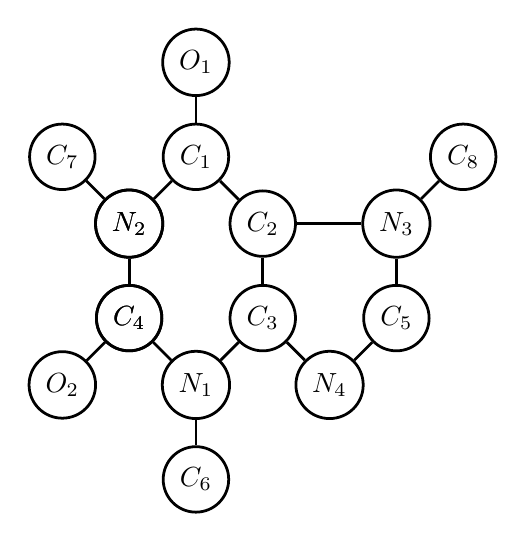
\begin{tikzpicture}[node distance={12mm}, line width=1pt, main/.style = {draw, circle}] 
\node[main] (1) []{$C_1$}; 
\node[main] (2) [below right of=1]{$C_2$}; 
\node[main] (3) [below of=2]{$C_3$}; 
\node[main] (4) [below left of=3]{$N_1$}; 
\node[main] (5) [above left of=4]{$C_4$}; 
\node[main] (6) [above of=5]{$N_2$};
\node[main] (9) [below right of=3]{$N_4$}; 
\node[main] (8) [above right of=9]{$C_5$}; 
\node[main] (7) [above of=8]{$N_3$}; 
\node[main] (10) [above of=1]{$O_1$}; 
\node[main] (11) [above left of=4]{$C_4$}; 
\node[main] (12) [above of=5]{$N_2$}; 

\node[main] (13) [below of=4]{$C_6$};  

\node[main] (17) [below left of=5]{$O_2$};

\node[main] (18) [above left of=6]{$C_7$}; 

\node[main] (22) [above right of=7]{$C_8$}; 



\draw [] (1) -- (2); 
\draw [] (2) -- (3); 
\draw [] (3) -- (4); 
\draw [] (4) -- (5); 
\draw [] (5) -- (6); 
\draw [] (6) -- (1); 
\draw [] (2) -- (7); 
\draw [] (7) -- (8); 
\draw [] (8) -- (9); 
\draw [] (9) -- (3); 
\draw [] (1) -- (10); 

\draw [] (4) -- (13); 

\draw [] (5) -- (17); 

\draw [] (6) -- (18); 

\draw [] (7) -- (22); 
\end{tikzpicture}
% \end{center}
}}
		\quad
		\subfloat[][A Path Decomposition]{\resizebox{0.16\textwidth}{!}{% !TEX root = ../main.tex
% \begin{center}
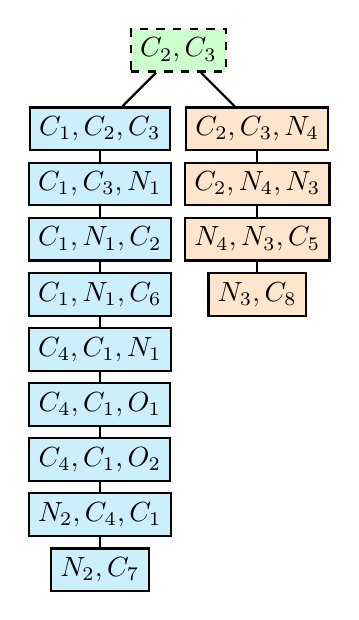
\begin{tikzpicture}[node distance={7mm}, thick, main/.style = {draw, rectangle}] 
\node[main, fill=green!20, dashed] at (0,0) (8) {$C_2,C_3$};
\node[main,fill=cyan!20] at (-1,-1) (7){$C_1,C_2,C_3$};
\node[main,fill=cyan!20] (100) [below of =7] {$C_1,C_3,N_1$};
\node[main,fill=cyan!20] (6) [below of =100]{$C_1,N_1,C_2$};
\node[main,fill=cyan!20] (5) [below of =6]{$C_1,N_1,C_6$};
\node[main,fill=cyan!20] (4) [below of =5]{$C_4,C_1,N_1$};
\node[main,fill=cyan!20] (3) [below of =4]{$C_4,C_1,O_1$};
\node[main,fill=cyan!20] (2) [below of =3]{$C_4,C_1,O_2$};
\node[main,fill=cyan!20] (1) [below of =2]{$N_2,C_4,C_1$};
\node[main,fill=cyan!20] (0) [below of =1] {$N_2,C_7$}; 

%\node[main,white] (00) [right = 1cm of 0] {}; 
%\node[main,white] (000) [left = 1cm of 0] {}; 



\node[main,fill=orange!20] at (1, -1) (9){$C_2,C_3,N_4$};
\node[main,fill=orange!20] (10) [below of =9]{$C_2,N_4,N_3$};
\node[main,fill=orange!20] (11) [below of =10]{$N_4,N_3,C_5$};
\node[main,fill=orange!20] (12) [below of =11]{$N_3, C_8$};


\draw [] (0) -- (1); 
\draw [] (1) -- (2); 
\draw [] (2) -- (3); 
\draw [] (3) -- (4); 
\draw [] (4) -- (5); 
\draw [] (5) -- (6); 
\draw [] (6) -- (100); 
\draw [] (7) -- (100); 
\draw [] (7) -- (8); 
\draw [] (8) -- (9); 
\draw [] (9) -- (10); 
\draw [] (10) -- (11); 
\draw [] (11) -- (12); 


\end{tikzpicture}
% \end{center}}}
		\quad
		\subfloat[][A Tree Decomposition]{\resizebox{0.3\textwidth}{!}{% \begin{center}
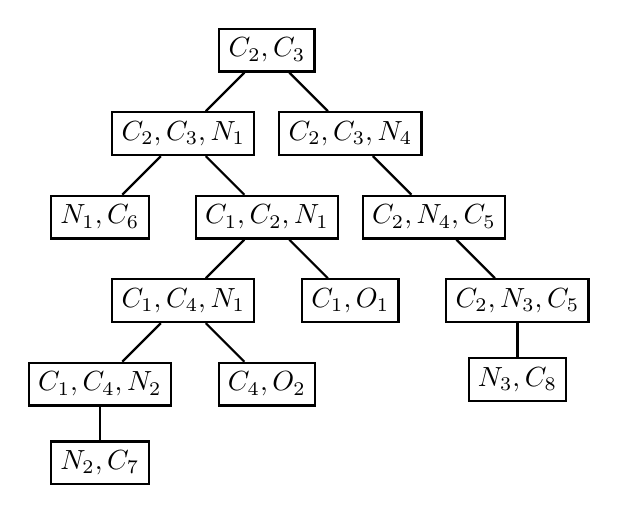
\begin{tikzpicture}[node distance={15mm}, thick, main/.style = {draw, rectangle}] 
\node[main] (0) []{$C_2,C_3$}; 
\node[main] (00) [below left of =0]{$C_2,C_3,N_1$};
\node[main] (000) [below left of =00]{$N_1,C_6$};
\node[main] (001) [below right of =00]{$C_1,C_2,N_1$};
\node[main] (0011) [below right of =001]{$C_1,O_1$};
\node[main] (0010) [below left of =001]{$C_1,C_4,N_1$};
\node[main] (00101) [below right of =0010]{$C_4,O_2$};
\node[main] (00100) [below left of =0010]{$C_1,C_4,N_2$};
\node[main] (001000) [below of =00100,,node distance={10mm}]{$N_2,C_7$};
\node[main] (01) [below right of =0]{$C_2,C_3,N_4$};
\node[main] (011) [below right of =01]{$C_2,N_4,C_5$};
\node[main] (0111) [below right of =011]{$C_2,N_3,C_5$};
\node[main] (01110) [below of =0111,,node distance={10mm}]{$N_3,C_8$};

\draw [] (0) -- (00); 
\draw [] (00) -- (000); 
\draw [] (00) -- (001); 
\draw [] (001) -- (0010); 
\draw [] (001) -- (0011); 
\draw [] (0010) -- (00100); 
\draw [] (00100) -- (001000);  
\draw [] (0010) -- (00101); 

\draw [] (0) -- (01); 
\draw [] (01) -- (011); 
\draw [] (011) -- (0111); 
\draw [] (0111) -- (01110); 

\end{tikzpicture}
% \end{center}}}
		\caption{A Graph Representation of Caffeine and a path and tree decomposition of this graph. Vertices in the root bag of the tree decomposition are highlighted in green (dashed). Notice how the removal of these nodes in the original molecule separates it into two connected components, each corresponding to one of the sides of the path decomposition, and one of the highlighted subtrees in the tree decomposition.}
		\label{fig:tree_dec_caffeine}
	\end{figure}

\end{example}
% \begin{figure}[H]
% 	\centerin{}g
% 	\chemfig{=^[:270](-[:330]=^[:30]-[:90]=^[:150]-[:210])-[:210]=_[:270](%
-[:330]=_[:30]-[:330]=_[:270]-[:210]=_[:150]-[:90])-[:210](-[:270]=_[:330]%
-[:270]=_[:210]-[:150]=_[:90]-[:30])=_[:150](-[:210]=_[:270]-[:210]=_[:150]%
-[:90]=_[:30]-[:330])-[:90](-[:150]=^[:90]-[:150]=^[:210]-[:270]=^[:330]%
-[:30])=_[:30](-[:330])-[:90]=^[:30]-[:90]=^[:150]-[:210]=^[:270](-[:330])}

% 	\caption{1,2,3,4,5,6-hexakis-phenylbenzene}
% 	\label{fig:tw_2 example}
% \end{figure}

\begin{lemma}[Proof in~\ref{app:proof}]\label{intseplemma}
	If $b$ is an introduce node with a single child $c$ and $X_b = X_c \cup \{v\}$, then $N(v)\cap G_b^\downarrow \subseteq X_c$. Here, $N(v)$ is the set of neighbors of $v.$
\end{lemma}



\begin{lemma}[Proof in~\ref{app:proof}]\label{joinseplemma}
	If $b$ is a join node with two children $c_1$ and $c_2,$ then in $G_b^\downarrow$ there is no edge with one endpoint in $V(G_{c_1}^\downarrow) \setminus X_b$ and the other in $V(G_{c_2}^\downarrow) \setminus X_b.$ Informally, $X_b$ is a cut that separates $V(G_{c_1}^\downarrow)$ from $V(G_{c_2}^\downarrow)$ in $G.$ See Figure~\ref{fig:tree_dec_caffeine}.
\end{lemma}

% \begin{proof}
% Let $T^\prime, T^{\prime\prime}, T^{\prime\prime\prime}$ be the subtrees of $T$ rooted at $b, c_1, c_2$ respectively. Let 
% $\mathcal{T}^\prime, \mathcal{T}^{\prime\prime}, \mathcal{T}^{\prime\prime\prime}$ be the corresponding tree decompositions. We will prove the given statement by contradiction. Therefore, let us assume that $u \in V(G_{c_1}^\downarrow) \setminus X_b$, $v \in V(G_{c_2}^\downarrow) \setminus X_b$, and $uv \in E(G_b^\downarrow)$.

% As $\mathcal{T}^{\prime}$ is a tree decomposition of $G^\downarrow_b$, there exists at least one bag $X_t$, such that $t \in \mathcal{T}^{\prime}$ and $u,v \in X_t$. From our initial assumption, we know that $u, v \notin X_b$, this implies that $t \neq b$. Therefore, either $t \in T^{\prime\prime}$ or $t \in T^{\prime\prime\prime}$. Without loss of generality, let us assume that $t \in T^{\prime\prime}$. As $v \in V(G_{c_2}^\downarrow) \setminus X_b$, there exists at least one bag $X_s$ such that, $ s \in T^{\prime\prime\prime}$ and $v \in X_s$. Observe that $v$ appears in both bags $X_s$ and $X_t$. Now by Definition \ref{def:tree_dec}, we know that $T^\prime_{v}$ is a connected subtree and any path connecting $s$ and $t$ goes through $b$. This implies that $X_b \in T^\prime_v$ and $v \in X_b$. This contradicts our initial assumption that $v \notin X_b$, hence completes the proof.
% \end{proof}

\section{Proofs} \label{app:proof}

\paragraph{Proof of Lemma~\ref{intseplemma}}
		Let $T^\prime$ be a subtree of the tree $T$ rooted at $b$. Observe that the corresponding tree decomposition
		$\mathcal{T}^\prime = \{T^\prime, \{X_t\}_{t\in V(T^\prime)}\}$ is a tree decomposition of $G_b^\downarrow$. Notice that by Definition \ref{def:tree_dec}, $T^\prime_v$ forms an induced subtree of the $T^\prime$. As $v \notin X_c$ and $c$ is the only vertex in the open neighborhood of $b$, this implies that $T^\prime_v = \{b\}$.
		Let $u$ be a vertex in $N(v) \cap G_b^\downarrow$, then by Definition \ref{def:tree_dec}, if there is an edge $uv$ in $G_b^\downarrow$, then there exists a bag containing both $u$ and $v$. But, as we have just shown that the only bag containing $v$ is $X_b$. As $u$ is a vertex in $N(v)$, this implies that $u \in X_c$.

\paragraph{Proof of Lemma~\ref{joinseplemma}}
	Let $T^\prime, T^{\prime\prime}, T^{\prime\prime\prime}$ be the subtrees of $T$ rooted at $b, c_1, c_2$ respectively. Let 
	$\mathcal{T}^\prime, \mathcal{T}^{\prime\prime}, \mathcal{T}^{\prime\prime\prime}$ be the corresponding tree decompositions. We will prove the given statement by contradiction. Therefore, let us assume that $u \in V(G_{c_1}^\downarrow) \setminus X_b$, $v \in V(G_{c_2}^\downarrow) \setminus X_b$, and $uv \in E(G_b^\downarrow)$.
	As $\mathcal{T}^{\prime}$ is a tree decomposition of $G^\downarrow_b$, there exists at least one bag $X_t$, such that $t \in \mathcal{T}^{\prime}$ and $u,v \in X_t$. From our initial assumption, we know that $u, v \notin X_b$, this implies that $t \neq b$. Therefore, either $t \in T^{\prime\prime}$ or $t \in T^{\prime\prime\prime}$. Without loss of generality, let us assume that $t \in T^{\prime\prime}$. As $v \in V(G_{c_2}^\downarrow) \setminus X_b$, there exists at least one bag $X_s$ such that, $ s \in T^{\prime\prime\prime}$ and $v \in X_s$. Observe that $v$ appears in both bags $X_s$ and $X_t$. Now by Definition \ref{def:tree_dec}, we know that $T^\prime_{v}$ is a connected subtree and any path connecting $s$ and $t$ goes through $b$. This implies that $X_b \in T^\prime_v$ and $v \in X_b$. This contradicts our initial assumption that $v \notin X_b$, hence completes the proof. 


\paragraph{Proof of Proposition~\ref{prop:comp_pw_perfmat}}
	At each bag, we have at most $2^{\pw}$ possibilities for $M.$ Thus, the total number of $\pma[\cdot,\cdot]$ values that need to be computed is $\bigO(n \cdot 2^\pw),$  each of which are computed in $\poly(\pw)$ time.
	
\paragraph{Proof of Proposition~\ref{prop:comp_tw_perfmat}}
	We only have to analyze the runtime at join nodes as the rest is similar to Proposition~\ref{prop:comp_pw_perfmat}. At each join node $b,$ we have to perform one step of the summation for each $M \subseteq X_b$ and each $H_1 \subseteq X_b \setminus M.$ This is because $H_2$ is uniquely determined by $H_1$ and $M.$ Consider a vertex $v \in X_b.$ The vertex $v$ is either in $M$ or in $H_1$ or in $H_2.$ Thus, it has three possibilities. Therefore, the total number of possible combinations of $M$ and $H_1$ is $3^{|X_b|} \leq 3^{\twi + 1}.$
	%The transition for a join node is the most expensive operation for this algorithm, the rest of the cases are similar to the dynamic programming on nice path decomposition in Section \ref{subsec:perfect_pathwidth}.
	%Note that the recurrence relation for the dynamic programming state of join node can be rewritten as:
	%\[
	%\sum_{H \subseteq X_b \setminus M}\pma[c_1,M\cup H]\cdot \pma[c_2, X_b \setminus H]
	%\]
	%
	%For each bag $X_b$ and for each $M \subseteq X_b$, we spend at most $\bigO(\poly(\twi)\cdot 2^{\lvert X_B \rvert - \lvert M \rvert})$ time. By using the binomial theorem, the total time spend for each bag $X_b$ for all possible subsets $M$ is $\bigO(\poly(\twi)\cdot 3^{\lvert X_B \rvert})$. It is known that there are at most $\bigO(n \cdot \twi)$ bags for any nice tree decomposition of $G$ \cite[Chapter 7]{cygan2015parameterized}. Therefore, we spend at most $\bigO(n\cdot \poly(\twi)\cdot3^{\twi})$ time to completely fill the dymamic programming table.


% \section{Proofs of Lemmas~\ref{intseplemma} and~\ref{joinseplemma}}\label{appendix:proof_intseplemma} 

% \paragraph{Proof of Lemma~\ref{intseplemma}}
%     Let $T^\prime, T^{\prime\prime}, T^{\prime\prime\prime}$ be the subtrees of $T$ rooted at $b, c_1, c_2$ respectively. Let 
%     $\mathcal{T}^\prime, \mathcal{T}^{\prime\prime}, \mathcal{T}^{\prime\prime\prime}$ be the corresponding tree decompositions. We will prove the given statement by contradiction. Therefore, let us assume that $u \in V(G_{c_1}^\downarrow) \setminus X_b$, $v \in V(G_{c_2}^\downarrow) \setminus X_b$, and $uv \in E(G_b^\downarrow)$.
%     As $\mathcal{T}^{\prime}$ is a tree decomposition of $G^\downarrow_b$, there exists at least one bag $X_t$, such that $t \in \mathcal{T}^{\prime}$ and $u,v \in X_t$. From our initial assumption, we know that $u, v \notin X_b$, this implies that $t \neq b$. Therefore, either $t \in T^{\prime\prime}$ or $t \in T^{\prime\prime\prime}$. Without loss of generality, let us assume that $t \in T^{\prime\prime}$. As $v \in V(G_{c_2}^\downarrow) \setminus X_b$, there exists at least one bag $X_s$ such that, $ s \in T^{\prime\prime\prime}$ and $v \in X_s$. Observe that $v$ appears in both bags $X_s$ and $X_t$. Now by Definition \ref{def:tree_dec}, we know that $T^\prime_{v}$ is a connected subtree and any path connecting $s$ and $t$ goes through $b$. This implies that $X_b \in T^\prime_v$ and $v \in X_b$. This contradicts our initial assumption that $v \notin X_b$, hence completes the proof. \qed



% \paragraph{Proof of Lemma~\ref{joinseplemma}}
%     Let $T^\prime, T^{\prime\prime}, T^{\prime\prime\prime}$ be the subtrees of $T$ rooted at $b, c_1, c_2$ respectively. Let 
%     $\mathcal{T}^\prime, \mathcal{T}^{\prime\prime}, \mathcal{T}^{\prime\prime\prime}$ be the corresponding tree decompositions. We will prove the given statement by contradiction. Therefore, let us assume that $u \in V(G_{c_1}^\downarrow) \setminus X_b$, $v \in V(G_{c_2}^\downarrow) \setminus X_b$, and $uv \in E(G_b^\downarrow)$.
%     As $\mathcal{T}^{\prime}$ is a tree decomposition of $G^\downarrow_b$, there exists at least one bag $X_t$, such that $t \in \mathcal{T}^{\prime}$ and $u,v \in X_t$. From our initial assumption, we know that $u, v \notin X_b$, this implies that $t \neq b$. Therefore, either $t \in T^{\prime\prime}$ or $t \in T^{\prime\prime\prime}$. Without loss of generality, let us assume that $t \in T^{\prime\prime}$. As $v \in V(G_{c_2}^\downarrow) \setminus X_b$, there exists at least one bag $X_s$ such that, $ s \in T^{\prime\prime\prime}$ and $v \in X_s$. Observe that $v$ appears in both bags $X_s$ and $X_t$. Now by Definition \ref{def:tree_dec}, we know that $T^\prime_{v}$ is a connected subtree and any path connecting $s$ and $t$ goes through $b$. This implies that $X_b \in T^\prime_v$ and $v \in X_b$. This contradicts our initial assumption that $v \notin X_b$, hence completes the proof. \qed



\section{Remaining Algorithms}
\label{sec:remalgo}

\subsection{Hosoya Index / Counting Matchings}\label{sec:matchings}

 We now turn to the problem of computing the Hosoya index of a molecular graph, i.e.~finding the number of all matchings in the graph.

\begin{definition}[Respectful Matchings]\label{def:respectful_matching}
	Let $\mathcal{P} = \{X_1, \dots X_r\}$ be a nice path decomposition of $G$. For each bag $b$ and each $M \subseteq X_b$, we define $\RM(b,M)$ as the set of all matchings $F$ in  $G_b^\downarrow \setminus M$ such that (i)~each matching edge $uv \in F$ has at least one endpoint in $G_b^\downarrow \setminus X_b,$ and (ii)~each vertex in $X_b \setminus M$ is covered by $F$. We further define $\ma[b, M] := |\RM(b,M)|.$
\end{definition}

\paragraph{Our Dynamic Programming Algorithm (Figures illustrating the algorithm steps are provided in \ref{appendix:figure_matching})}
Given that $X_r = \emptyset$ is the root node, we have $G_{r}^\downarrow = G$, and all matchings of $G$ are in $\RM(r,\emptyset)$, which implies $\ma [r, \emptyset]$ is the Hosoya index of $G$. As in the previous section, we provide a bottom-up dynamic programming algorithm handling each type of node as follows:
\begin{compactitem}
	\item \textbf{Leaf Nodes:} If $X_l$ is a leaf bag then $\RM(l,M)$ contains only the empty matching as $X_l = \emptyset$. Therefore, $\ma[l,\emptyset] = 1$.
	\item \textbf{Introduce Nodes:} If $b$ introduces $v$ and has a child $c,$ we have: 
	\[
	\ma [b,M] =
	\begin{cases}
		\ma [c,M\setminus \{v\}] &v \in M\\
		0 &v \not\in M
	\end{cases}.
	\]
	In order to derive the above recurrence relation, we consider two possibilities for $v$:
	\begin{compactenum}
		\item If $v \in M$, then by Definition \ref{def:respectful_matching}, the matchings in $\RM(b,M)$ are the same as those in $\RM(c, M \setminus v)$. 
		\item If $v \notin M$, then for every matching $F \in \RP(b,M)$, $v$ should be covered by some edge $vw \in F$. By Lemma \ref{intseplemma}, $w \in X_{c} \subset X_b$, which contradicts the Definition \ref{def:respectful_matching}. Therefore, $\ma[b,M] = 0.$ for this case.
	\end{compactenum}
	
	%This transition from $X_c$ to $X_b$ can be computed in $\bigO(1)$ time. 
	
	\item \textbf{Forget Nodes:} Let $b$ be a forget node such that $X_b = X_c \setminus \{v\}$. We have:
	\[
	\ma[b,M]= \ma[c, M] +  \ma[c, M \cup \{v\}] \\
	+ \sum_{u \in X_b\setminus M:\ uv\in E(G)}\ma[c, M \cup \{u, v\}].
	\]
	
	This is obtained by a similar argument as in the case of perfect matchings. Every matching in $\RM(b, M)$ is in one of three cases. It either (i)~matches $v$ with a vertex outside $X_c,$ or (ii)~does not match $v$, or (iii)~matches $v$ with another vertex $u$ in $X_c.$ The matchings in (i) and (ii) are precisely those in $\RM(c, M)$ and $\RM(c, M \cup \{v\}),$ respectively, by Definition~\ref{def:respectful_matching}. For part (iii), if $v$ is matched with $u,$ then we should not match either of them to any other vertex. Thus, what remains is a matching in $\RM(c, M \cup \{u, v\}).$
	
	% \[
	% \ma[b,M]=
	% \ma[c, M] + \ma[c, M \cup \{v\}] + \sum_{u \in X_b\setminus M:\ uv\in E(G)}\ma[c, M \cup \{v,u\}]
	% \]
	%In order to derive the above recurrence relation, let $F$ be a matching from the set $\RM(b,M)$. Note that $v \notin M$, as $M \subseteq X_b$. There are two possibilities for $v$ i.e., either it will be covered by some edge in $F$ or it remains unmatched. For the latter case, all such matchings $F$ for which $v$ remains unmatched are in one-to-one correpondence with all matchings of the set $\RM(c,M\cup\{v\}$, and number of such matchings correspond to the second term $\ma[c, M \cup \{v\}]$ of the recurrsion. Now let us consider the second case, where $v$ will be matched by some edge $uv \in F$. Now there are again two possible cases to consider i.e., either $u \notin X_b$ or $u \in X_b$. For the former case when $u \notin X_b$, it is clear that there is a bijection between all such matchings $F$ and all elements of $\RM(c,M)$. Therefore, number of such matchings correspond to the first term $\ma[c,M]$ of the recurrence relation. Now let's consider the latter case when $u \in X_b$, then the matching $F \setminus uv \in \RM(c,M M \cup \{u, v\})$, and number of such matchings correspond to the last term $\sum_{u \in X_b\setminus M:\ uv\in E(G)}\ma[c, M \cup \{v,u\}]$ of the recurrence relation.
	
	
	% To prove that consider any $(X_b, M)$-respectful matching $F$. If $v$ unmached, $v \notin V(F)$ and $F$ is $(X_c, M \cup \{v\})$-respectful. If $v$ is matched with some vertex $u$, we have two cases:  either $w \notin X_b$ $w \in X_b$. In a first case the mathching $F$ is $(X_c, M)$-respectful, and this case corresponds to the term $\dpt[c, M \cup \{v\}]$. If $w \in X_b$, then exist edge $uv$ and matching $F \setminus uv$ is $(X_c, M \cup \{v, u\})$-respectful, which corresponds to the sum of $\dpt[c, M\cup \{v, u\}]$ terms. All correspondences is one-to-one.  
	
	
	% To prove that consider any $(X_b, M)$-respectful matching $F$. Since $v \notin M$, $v$ should be matched with some point, say, $u$. Then if $u\notin X_b$, matching $F$ is $(X_{c}, M)$-respectful, and number of such cases corresponds to the first term. If $u \in X_b$ then mathching $F \setminus uv$ is $(X_{c}, M \cup \{u, v\})$ respectful and correspondence is one-to-one.  
	
	%This transition to $X_b$ can be computed in $\bigO(\lvert X_b\rvert) = \bigO(\pw(G))$ time.
\end{compactitem}

% \begin{figure}[h]
	% \caption{Computing values in forget nodes. Cases for introduce and merge nodes are the same as to \ref{subsec:perfect_pathwidth}, represented in \ref{fig:introduce_node} and \ref{fig:join_node}, respectively. Forget nodes need to consider one more case when compared to \ref{fig:forget_node}, represented by the second case below bag $b$. This is when $x_1$ remains unmatched, since we do not need to generate a perfect matching.
		% }\label{fig:forget_node_matching}
	% {\resizebox{0.63\textwidth}{!}{% !TEX root = ../main.tex
\begin{tikzpicture}[line width=1pt,node distance=14mm ,main/.style = {draw, rectangle},scale=1] 

    \node[scale=.8] at (3.15,6){$\textup{Match}[b,\{x_4\}]$};
       
       \node[main] at (3.15,4.5) (9) {
   \begin{tikzpicture}[line width=1pt,node distance=14mm ,main/.style = {draw, circle},scale=1] 
   \node[main,color=black] at (1,1) (x2) {\texttt{$x_2$}};
       \node[main,color=black] at (0,0) (x3) {\texttt{$x_3$}};
       \node[main,fill=blue!40!white,densely dashed] at (1,0) (x4) {\texttt{$x_4$}};
      \draw (x2) -- (x3);
      \draw (x3) -- (x4);
   \end{tikzpicture}
       };
       
    \node[scale=.8] at (-1.5,1.5){$\textup{Match}[c,\{x_4\}]$};
       \node[main] at (-1.5,0) (8) {
   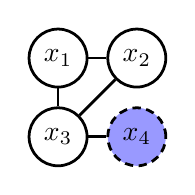
\begin{tikzpicture}[line width=1pt,node distance=14mm ,main/.style = {draw, circle},scale=1] 
   \node[main,color=black] at (0,1) (x1) {\texttt{$x_1$}};
   \node[main,color=black] at (1,1) (x2) {\texttt{$x_2$}};
       \node[main,color=black] at (0,0) (x3) {\texttt{$x_3$}};
       \node[main,fill=blue!40!white,densely dashed] at (1,0) (x4) {\texttt{$x_4$}};
      \draw (x1) -- (x2);
       \draw (x1) -- (x3);
      \draw (x2) -- (x3);
      \draw (x3) -- (x4);
   \end{tikzpicture}
   };
   
    \node[scale=.8] at (1.3,1.5){$\textup{Match}[c,\{x_4\}\cup \{x_1\}]$};
   \node[main] at (1.3,0) (8) {
   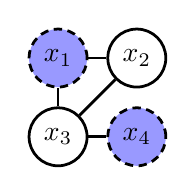
\begin{tikzpicture}[line width=1pt,node distance=14mm ,main/.style = {draw, circle},scale=1] 
   \node[main,fill=blue!40!white,densely dashed] at (0,1) (x1) {\texttt{$x_1$}};
   \node[main,color=black] at (1,1) (x2) {\texttt{$x_2$}};
       \node[main] at (0,0) (x3) {\texttt{$x_3$}};
       \node[main,fill=blue!40!white,densely dashed] at (1,0) (x4) {\texttt{$x_4$}};
      \draw (x1) -- (x2);
       \draw (x1) -- (x3);
      \draw (x2) -- (x3);
      \draw (x3) -- (x4);
   \end{tikzpicture}
   };
   
    \node[scale=.8] at (4.5,1.5){$\textup{Match}[c,\{x_4\}\cup \{x_1,x_2\}]$};
   \node[main] at (4.5 ,0) (8) {
   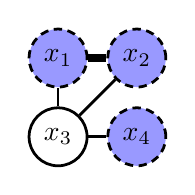
\begin{tikzpicture}[line width=1pt,node distance=14mm ,main/.style = {draw, circle},scale=1] 
   \node[main,fill=blue!40!white,densely dashed] at (0,1) (x1) {\texttt{$x_1$}};
   \node[main,fill=blue!40!white,densely dashed] at (1,1) (x2) {\texttt{$x_2$}};
       \node[main,color=black] at (0,0) (x3) {\texttt{$x_3$}};
       \node[main,fill=blue!40!white,densely dashed] at (1,0) (x4) {\texttt{$x_4$}};
      \draw [line width = 3pt, color=black]  (x1) -- (x2);
       \draw (x1) -- (x3);
      \draw (x2) -- (x3);
      \draw (x3) -- (x4);
   \end{tikzpicture}
   };

   \node[scale=.8] at (7.8,1.5){$\textup{Match}[c,\{x_4\}\cup \{x_1,x_3\}]$};
   \node[main] at (7.8,0) (8) {
   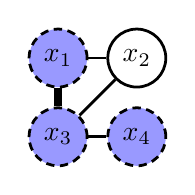
\begin{tikzpicture}[line width=1pt,node distance=14mm ,main/.style = {draw, circle},scale=1] 
   \node[main,fill=blue!40!white,densely dashed] at (0,1) (x1) {\texttt{$x_1$}};
   \node[main,color=black] at (1,1) (x2) {\texttt{$x_2$}};
       \node[main,fill=blue!40!white,densely dashed] at (0,0) (x3) {\texttt{$x_3$}};
       \node[main,fill=blue!40!white,densely dashed] at (1,0) (x4) {\texttt{$x_4$}};
      \draw (x1) -- (x2);
       \draw [line width = 3pt, color=black] (x1) -- (x3);
      \draw (x2) -- (x3);
      \draw (x3) -- (x4);
   \end{tikzpicture}
   };
   
       \draw [decorate,decoration={brace,amplitude=10}] (-1.5,2.5) -- (7.8,2.5) node [black,midway,xshift=-0.6cm] {};
   
       %\node[text width=6cm] at (2,-2){$\DP[i,c]$};
       %\node[text width=6cm] at (5.5,-2){$\DP[i,c+\{x_4\to \texttt{gray/dotted}]$};
      
   \end{tikzpicture}
   }}
	% \end{figure}


\begin{proposition}\label{prop:comp_pw_mat}
	
	Given a graph $G$ with $n$ vertices and a nice path decomposition $\mathcal{P} $ of $G$ with $O(n)$ bags and width $\pw,$ the algorithm above finds the Hosoya index, i.e.~the total number of matchings, in time $\bigO(n\cdot \poly(\pw) \cdot2^{\pw}).$
\end{proposition}
\begin{proof}
	The runtime analysis is identical to Proposition \ref{prop:comp_pw_perfmat}.
	% For each bag, we have atmost $2^{\pw}$ dynamic programming states, and for each state we spend atmost $\bigO(\poly(\pw))$ time. It is known that there are atmost $\bigO(n)$ bags for any nice path decomposition of $G$ \cite[Chapter 7]{cygan2015parameterized}. Therefore, we spend atmost $\bigO(n\cdot \poly(\pw) \cdot2^{\pw})$ time to completely fill the dymamic programming table.
\end{proof}

%\subsubsection{Bounded Treewidth}\label{subsec:matching_treewidth}
%% We will use a dynamic programming approach over the nice tree decomposition of the given graph $G$. The definitions of respectful matchings and dynamic programming states used here are same as Section \ref{sec:pathwidth_matchings}. Let $\mathcal{T} = \{T, \{X_t\}_{t \in V(T)}\}$ be a nice tree decomposition of the graph $G = (V,E)$ under consideration.
%
%% We will use a dynamic programming over the nice tree decomposition. Definitions of dynamic programming and respectfulness have only cosmetic differences with path decomposition case. Let us fix a nice tree decomposition $\mathcal{T} = \{T, \{X_t\}_{t \in V(T)}\}$. For each $b \in T$ and each $M \subseteq X_b$ we will define $\dpt[b, M]$ as a number of perfect matchings in a $G_b^\downarrow \setminus M$ such that each matching edge $uv$ has at least on point in $G_b^\downarrow \setminus X_b$: $u \notin X_b$ or $v \notin X_b$. We call such matchings \textit{respectful} to the $(X_b, M)$.
%
%
%% \begin{remark}
	%
	%% \end{remark}
%% If $X_l = \varnothing$ is a leaf bag, we have only empty $(X_l, \varnothing)$-respectful matching, which means 
%% \[
%% 	\dpt[X_l, \varnothing] = 1.
%% \]
%
%% Also for the root bag $X_r$, $\dpt[X_r, \varnothing]$ contains number of perfect matchings in a whole graph $G$.
%
%
%% Cases of introduce and forget nodes repet verbatim. We need only consider merge case now. 
%% We now provide a bottom-up approach for filling up the dynamic table. The dynamic table relations depend on the type of the bag. There are four possible cases for the type of bags, i.e., when $X_b$ is: leaf node, introduce node, forget node and join node 
%respectively. 
%The reccurrence relations for leaf node, introduce node and forget node remains the same as Section \ref{sec:pathwidth_matchings}. Therefore, we only need to consider the case of join node which is described as follows:

\paragraph{Extension to Tree Decompositions} As in the previous section, in order to extend our algorithm to tree decompositions, we only need to specify how to handle join nodes in our bottom-up dynamic programming:
\begin{compactitem}
	\item \textbf{Join Nodes:} Let $b$ be a join node with ${c_1}$ and ${c_2}$ as its children. We then have:
	\[
	\ma[b,M] = \sum_{H_1 \sqcup H_2 = X_b \setminus M}\ma[c_1,M\cup H_2]\cdot \ma[c_2, M\cup H_1].
	% \\
	% &=\sum_{H \subseteq X_b \setminus M}\pma[c_1,M\cup H]\cdot \pma[c_2, X_b \setminus H],\\
	\]
	
	where $H_1 \sqcup H_2 = X_b \setminus M$ means $H_1 \cup H_2 = X_b \setminus M$ and $H_1 \cap H_2 = \emptyset$. 
	% This two formulas yields same result, but first easier to analyze and second easier to implement.  
	In order to derive the above recurrence relation, let $F$ be a matching from the set $\RM(b,M)$. By Lemma~\ref{joinseplemma}, $F$ does not have any edges between $G_{c_1}^\downarrow \setminus X_b$ and $G_{c_2}^\downarrow \setminus X_b$. Therefore, it can be split into two matchings, $F_1 := E(G_{c_1}^\downarrow) \cap F$ and $F_2 := E(G_{c_2}^\downarrow) \cap F$. Let $H_1 := V(F_1) \cap X_b$ and $H_2 := V(F_2) \cap X_b$. Following Definition \ref{def:respectful_matching}, we have $F_1 \in \RM(c_1,M \cup H_2)$ and $F_2 \in \RM(c_2,M \cup H_1)$. If we choose $H_1$ and $H_2$ such that $H_1 \sqcup H_2 = X_b \setminus M$, then for all such matchings $F_1 \in \RM(c_1,M\cup H_2)$ and $F_2 \in \RM(c_2, M\cup H_1)$, we get a matching $ F = F_1 \cup F_2$, such that $F \in \RM(b,M)$. %This leads to our recurrence relation.
	
	
	% Consider arbitrary $(X_b, M)$-respectful matching $F$. By lemma \ref{joinseplemma} $F$ do not have edges between $G_{c_1}^\downarrow \setminus X_b$ and $G_{c_2}^\downarrow \setminus X_b$. Let us split this matching $F$ into $F_1 := E(G_{c_1}^\downarrow) \cap F$, $F_2 := E(G_{c_2}^\downarrow) \cap F$, also let $H_1 := V(F_1) \cap X_b$, $H_2 := V(F_2) \cap X_b$. Observe that $F_1$ is $(X_{c_1}, M \cup H_2)$-respectful and $F_2$ is $(X_{c_2}, M \cup H_1)$-respectful. Notice that if $H_1, H_2$ are chosen, $F_1, F_2$ acts independently, so when $H_1, H_2$ fixed such matching could be counted as $\dpt[c_1, M \cup H_2] \cdot \dpt[c_2, M \cup H_1]$, which leads to our formula. 
	
\end{compactitem}

\begin{proposition}\label{prop:comp_tw_match}
	
	Given a graph $G$ with $n$ vertices and a nice tree decomposition $\mathcal{T}$ of $G$ with $O(n)$ bags and width $\twi,$ the algorithm above finds the total number of perfect matchings, i.e.~the Hosoya index, in time $\bigO(n\cdot \poly(\twi)\cdot3^{\twi})$.
	
	%The time complexity for finding the total number of matchings for a graph $G = (V,E)$, with $\lvert V \rvert = n$ and treewidth $\twi$, using the above algorithm is $\bigO(n\cdot \poly(\twi)\cdot3^{\twi})$.
	% With this, the final complexity of the algorithm increases to .
\end{proposition}
\begin{proof}
	The runtime analysis is identical to \ref{prop:comp_tw_perfmat}.
	% The transition for a join node is the most expensive operation for this algorithm, the rest of the cases are similar to the dynamic programming on nice path decomposition in Section \ref{subsec:perfect_pathwidth}.
	% Note that the recurrence relation for the dynamic programming state of join node can be rewritten as:
	% \[
	% \sum_{H \subseteq X_b \setminus M}\pma[c_1,M\cup H]\cdot \pma[c_2, X_b \setminus H]
	% \]
	
	% For each bag $X_b$ and for each $M \subseteq X_b$, we spend atmost $\bigO(\poly(\twi)\cdot 2^{\lvert X_B \rvert - \lvert M \rvert})$ time. By using binomial theorem, the total time spend for each bag $X_b$ for all possible subsets $M$ is $\bigO(\poly(\twi)\cdot 3^{\lvert X_B \rvert})$. It is known that there are atmost $\bigO(n)$ bags for any nice path decomposition of $G$ \cite[Chapter 7]{cygan2015parameterized}. Therefore, we spend atmost $\bigO(n\cdot \poly(\twi)\cdot3^{\twi})$ time to completely fill the dymamic programming table.
\end{proof}


% \subsection{Bounded Treewidth}

% Again we will use a dynamic programming over the nice tree decomposition in a bottom-up manner. Let us fix a nice tree decomposition $\mathcal{T} = \{T, \{X_t\}_{t \in V(T)}\}$. For each node $b$ and each subset of a bag $M \subset X_b$ we define $\dpt[b, M]$ as a number of matchings in a $G_b^\downarrow \setminus M$ such that each matching edge $uv$ has at least on point in $G_b^\downarrow \setminus X_b$: $u \notin X_b$ or $v \notin X_b$ and each point from $X_b \setminus M$ is covered. We call such matchings \textit{respectful} to the $(X_b, M)$.


% % If $X_l = \varnothing$ is a leaf bag, we have only empty $(X_l, \varnothing)$-respectful matching, which means 
% % \[
% % \dpt[X_l, \varnothing] = 1.
% % \]

% % Also for the root bag $X_r$, $\dpt[X_r, \varnothing]$ contains number of matchings in a whole graph $G$.

% % Now we need to consider three cases of tree decomposition nodes: introduce node, forget node and merge node. 

% % \textbf{Introduce case.} Let $X_b$ is an introduce bag which introduces vertex $v$, let its child is a bag $X_c$, $X_b = X_c \cup \{v\}$. Then  
% % \[
% % \dpt[b,M] =
% % \begin{cases}
	% % \dpt[c,M\setminus v], &v \in M,\\
	% % 0, &v \not\in M.
	% % \end{cases}
% % \]
% % Indeed, if $v \in M$, we need to count respectful matchings to the $(X_b, M)$, but that matchings in one-to-one correspondance with respectful matchings to $(X_c, M \setminus v)$. On the other hand, if $v \notin M$, consider any $(X_b, M)$-respectful matching. In that matching $v$ should be covered by some edge $vw$. By lemma \ref{intseplemma}, $w \in X_{c} \subset X_b$, which contradicts with definition of of being respectful. 

% % This transition can be calculated in $\bigO(1)$ time. 

% % \textbf{Forget case.} Consider now a node $X_b$. Let $v$ be the vertex erased in $X_b$ and $X_c$ is a child of the $X_b$. Then

% % \[
% % \dpt[b,M]=
% % \dpt[c, M] + \dpt[c, M \cup \{v\}] + \sum_{u \in X_b\setminus M:\ uv\in E(G)}\dpt[c, M \cup \{v,u\}].
% % \]

% % To prove that consider any $(X_b, M)$-respectful matching $F$. If $v$ unmached, $v \notin V(F)$ and $F$ is $(X_c, M \cup \{v\})$-respectful. If $v$ is matched with some vertex $u$, we have two cases:  either $w \notin X_b$ $w \in X_b$. In a first case the mathching $F$ is $(X_c, M)$-respectful, and this case corresponds to the term $\dpt[c, M \cup \{v\}]$. If $w \in X_b$, then exist edge $uv$ and matching $F \setminus uv$ is $(X_c, M \cup \{v, u\})$-respectful, which corresponds to the sum of $\dpt[c, M\cup \{v, u\}]$ terms. All correspondences is one-to-one.  

% % This transition can be calculated in $\bigO(\lvert X_b\rvert) = \bigO(\textup{tw}(G))$ time.

% \textbf{Merge case}. Consinder merge node $X_b$ and two its children $X_{c_1}$ and $X_{c_2}$, $X_b = X_{c_1} = X_{c_2}$.
% We claim that
% \[
% \begin{split}
	% \dpt[b,M] &= \sum_{H_1 \sqcup H_2 = X_b \setminus M}\dpt[c_1,M\cup H_2]\cdot \dpt[c_2, M\cup H_1]\\
	% &=\sum_{H \subseteq X_b \setminus M}\dpt[c_1,M\cup H]\cdot \dpt[c_2, X_b \setminus H],\\
	% \end{split}
% \]

% where $H_1 \sqcup H_2 = X_b \setminus M$ means $H_1 \cup H_2 = X_b \setminus M$ and $H_1 \cap H_2 = \varnothing$.  

% Consider arbitrary $(X_b, M)$-respectful matching $F$. By lemma \ref{joinseplemma} $F$ do not have edges between $G_{c_1}^\downarrow \setminus X_b$ and $G_{c_2}^\downarrow \setminus X_b$. Let us split this matching $F$ into $F_1 := E(G_{c_1}^\downarrow)\cap F$, $F_2 := E(G_{c_2}^\downarrow) \cap F$, also let $H_1 := V(F_1) \cap X_b$, $H_2 := V(F_2) \cap X_b$. Observe that $F_1$ is $(X_{c_1}, M \cup H_2)$-respectful and $F_2$ is $(X_{c_2}, M \cup H_1)$-respectful. Notice that if $H_1, H_2$ are chosen, $F_1, F_2$ acts independently, so when $H_1, H_2$ fixed, such matchings could be counted as $\dpt[c_1, M \cup H_2] \cdot \dpt[c_2, M \cup H_1]$, which leads to our formula. 


% \begin{proposition}
	% The final complexity is $\bigO(n\cdot \textup{tw}\cdot3^{\textup{tw}})$
	
	% \end{proposition} 


\subsection{Counting Matchings of All Sizes}\label{sec:entropy_matchings}

In this section, given a graph $G$ and a tree/path decomposition, our goal is to find the number of matchings of size $k$ in $G$ for every $k.$
We need to only slightly adapt the dynamic programming values defined in Section~\ref{sec:matchings}, in order to count matchings of each size separately. The derivation of recurrence relations and their correctness is also very similar to Section~\ref{sec:matchings}. Finally, given this information, computing the entropy is a simple matter of applying Equation~\eqref{eq:entropy}.



\begin{definition}[Respectful Matchings of size $k$]\label{def:respectful_matching_size_k}
Given a nice path decomposition $\mathcal{P} = \{X_1, \dots X_r\}$ of $G,$ for each bag $b$ and each $M \subseteq X_b$, we define $\RM(b,k,M)$ as the set of all matchings $F$ in  $G_b^\downarrow \setminus M$ such that (i)~$\lvert F \rvert = k$; (ii)~each matching edge $uv \in F$ has at least one endpoint in $G_b^\downarrow \setminus X_b$; and (iii)~every vertex in $X_b \setminus M$ is covered by $F$. We further define $\ma[b,k,M] := |\RM(b,k,M)|.$
\end{definition}

\paragraph{Our Dynamic Programming Algorithm} Since $X_r = \emptyset$ is the root node, $G_{r}^\downarrow = G$, and $\ma [r, k,\varnothing]$ counts matchings of size $k$ in $G$. We process the bags in a bottom-up order as follows:
% If $X_l = \varnothing$ is a leaf bag, only $(X_l, \varnothing)$-respectful matching is an empty 
% matching, which means: 
% \[
% \dpt[X_l, \varnothing] = 1.
% \]


% We now provide a bottom-up approach for filling up the dynamic table. The dynamic table relations depend on the type of the bag. We need to consider three cases when $X_b$ is: leaf node, introduce node and forget node respectively.
\begin{compactitem}
\item \textbf{Leaf Nodes:} If $X_l$ is a leaf bag then $\RM(l,k,M)$ contains only the empty matching as $X_l = \emptyset$. Therefore, $\ma[l,0,\emptyset] = 1$ and for any other $k > 0$ $\ma[l,k,\emptyset] = 0$.
\item \textbf{Introduce Nodes:} If $b$ introduces $v$ and has a single child $c$ then, we have:
\[
\ma [b,k,M] =
\begin{cases}
\ma [c,k,M\setminus v] &v \in M\\
0 &v \not\in M
\end{cases}.
\]

\item \textbf{Forget Nodes:} Let $b$ be a forget node with child $c$ and $X_b = X_c \setminus \{v\}$, then
\[
\ma[b,k,M]= \ma[c,k,M] +  \ma[c,k,M \cup \{v\}] 
+ \sum_{u \in X_b\setminus M:\ uv\in E(G)}\ma[c,k-1, M \cup \{u, v\}].
\]

\end{compactitem}

\begin{proposition}\label{prop:comp_pw_matchings_size_k} \label{prop:twe}
	
		Given a graph $G$ with $n$ vertices and a nice path decomposition $\mathcal{P} $ of $G$ with $O(n)$ bags and width $\pw,$ the algorithm above finds the number of matchings of size $k$ for every $0 \leq k \leq \frac{n}{2}$ in time $\bigO(n^2 \cdot \poly(\pw) \cdot2^{\pw}).$
	
%The time complexity for finding the total number of matchings of all possible sizes for a graph $G = (V,E)$, with $\lvert V \rvert = n$ and pathwidth $\pw$, using the above algorithm is $\bigO(n^2\cdot \poly(\pw) \cdot2^{\pw})$.
%% The final complexity is $\bigO(n\cdot \textup{pw}\cdot2^{\textup{pw}})$
\end{proposition}
\begin{proof}
The analysis is similar to that of Proposition~\ref{prop:comp_pw_perfmat}, except that we now have $O(n)$ times as many dynamic programming values, one for each value of $k.$
\end{proof}
%\subsubsection{Bounded Treewidth}\label{sec:entropy_matchings_tw}
% We will use a dynamic programming approach over the nice tree decomposition of the given graph $G$. The definitions of respectful matchings of fixed size and dynamic programming states used here are same as Section \ref{sec:entropy_matchings_pw}. Let $\mathcal{T} = \{T, \{X_t\}_{t \in V(T)}\}$ be a nice tree decomposition of the graph $G = (V,E)$ under consideration.

%% We now provide a bottom-up approach for filling up the dynamic table. The dynamic table relations depend on the type of the bag. There are four possible cases for the type of bags, i.e., when $X_b$ is: leaf node, introduce node, forget node and join node respectively. 
%The reccurrence relations for leaf node, introduce node and forget node remains the same as Section \ref{sec:entropy_matchings_pw}. Therefore, we only need to consider the case of join node which is described as follows:

\paragraph{Extension to Tree Decompositions} 
If the input contains a tree decomposition rather than a path decomposition, our algorithm proceeds in a bottom-up order and handles the join nodes as follows:
\begin{compactitem}
	\item \textbf{Join Nodes:} 
	Let $b$ be a join node with children ${c_1}$ and ${c_2}.$ We define $n_b := \lvert V(G_b^{\downarrow}) \rvert$. We define $n_{c_1}$ and $n_{c_2}$ similarly and, without loss of generality, assume that $n_{c_1} \leq n_{c_2}$\footnote{If $n_{c_1} = n_{c_2}$ we choose the lexicographically smaller bag as $c_1.$}. We call $c_1$ the \emph{light} child of $b$ and $c_2$ the \emph{heavy} child. We also note that 
	\begin{equation} \label{eq:oneandhalf} n_b = n_{c_1} + n_{c_2} - |X_b| \geq 2 \cdot n_{c_1} - |X_b|.
\end{equation}
Finally, we have:
\begin{equation} \label{eq:joinmatch}
\hspace{-1cm}\ma[b,k,M] = 
\sum_{0\leq k_{1}\leq \frac{n_{c_1}}{2}} \sum_{H_1 \sqcup H_2 = X_b \setminus M}\ma[c_1,k_{c_1},M\cup H_2]\cdot \ma[c_2,k-k_1, M\cup H_1].
\end{equation}
\end{compactitem}
This is similar to Section~\ref{sec:matchings}, except that we choose to explicitly keep track of the number of matching edges that come from $G^\downarrow_{c_1},$ i.e.~$k_1,$ and the other $k-k_1$ edges of the matching come from $G^\downarrow_{c_2}.$ Note that the first sum above is on $n_{c_1}$ where $c_1$ was the light child of $b.$


% We refer the reader to \ref{appendix:figure_matching} for figures illustrating the dynamic programming algorithm described above.


%\begin{lemma}\label{lem:technical_lemma_for_matching_entropy}
%Let $\mathcal{T} = \{T, \{X_t\}_{t \in V(T)}\}$ be a nice tree decomposition of the graph $G = (V,E)$. Then $\sum n_a$ for all smaller subtrees $T_a$ in $\SSt(\mathcal{T})$ is at most $\bigO(n\cdot \log n)$.
%
%% Then $ \sum_{T_a \in \SSt(\mathcal{T})} n_a$ is atmost $\bigO(n\cdot log(n))$.
%\end{lemma}
%\begin{proof}
%Let $x_v$ be the number of times any vertex $v$ appears in the smallest subtree of some node with more than one child.
%
%\[\sum_{T_a \in \SSt(\mathcal{T})}n_a = \sum_{v\in T} x_v \]
%
%Observe that $v$ can have at most $\log n$ ancestors with degree more than two in which it is part of the smallest subtree.
%
%This can be shown by keeping track of the current subtree and iterating through the ancestors of $v$. Every time $v$ is in the smallest subtree of a node with more than one child, the size of such subtree doubles, and this can happen at most $\log n$ times.
%
%Therefore, we get the following bound on number of vertices for all smaller subtrees:
%\[
%\sum_{T_a \in \SSt(\mathcal{T})}n_a = \sum_{v\in T} x_v \leq \sum_{v\in T} \log n \leq n \log n
%\]
%\end{proof}

% \begin{figure}[h]
% \resizebox{0.32\textwidth}{!}{% !TEX root = ../main.tex
% \begin{center}
\begin{tikzpicture}[node distance={17mm}, thick, main/.style = {draw, rectangle split,rectangle split parts=2}] 
\node[main] (0) []{ $n_b = 72$ \nodepart{two}$x_1,x_2,x_3$}; 
\node[main] (00) [below left of =0]{ $n_b = 40$ \nodepart{two}$x_1,x_2,x_3$};
\node[] (000) [below of =00,node distance={8mm}]{...};

\node[main,fill=cyan!20, dashed] (01) [below right of =0]{$n_b = 35$ \nodepart{two}$x_1,x_2,x_3$};
\node[] (010) [below of =01,node distance={8mm}]{...};
\node[main] (011) [below of =010,node distance={8mm}]{$n_b = 29$ \nodepart{two}$x_1,x_{10},x_{11}$};
\node[main] (0110) [below left of =011]{$n_b = 20$ \nodepart{two}$x_1,x_{10},x_{11}$};
\node[] (0110p) [below of =0110,node distance={8mm}]{...};
\node[main,fill=cyan!20, dashed] (0111) [below right of =011]{$n_b = 12$ \nodepart{two}$x_1,x_{10},x_{11}$};
\node[] (0111p) [below of =0111,node distance={8mm}]{...};
\node[main] (01110) [below of =0111p,,node distance={8mm}]{$n_b = 6$ \nodepart{two}$x_{10},\textcolor{red}{x_{15}}$};
\node[] (01110p) [below of =01110,node distance={8mm}]{...};

\draw [] (0) -- (00); 
\draw [] (00) -- (000); 

\draw [line width=3pt] (0) -- (01); 
\draw [] (01) -- (010); 
\draw [] (010) -- (011); 

\draw [line width=3pt] (011) -- (0111); 
\draw [] (011) -- (0110); 
\draw [] (0110) -- (0110p); 

\draw [] (0111) -- (0111p); 
\draw [] (0111p) -- (01110); 

\draw [] (01110) -- (01110p); 


\end{tikzpicture}
% \end{center}}
% \caption{This figure illustrates Proposition \ref{prop:comp_tw_matchings_size_k}. The tree shown represents a nice tree decomposition. Sequences of forget and introduce nodes have been omitted by ``...''. Bags in $L$, or bags that are the light child of some join bag, have been highlighted in blue (dashed). Notice that each of these bags has a parent $b$ with weight $n_b$ at least $1.5$ times the weight of its lightest child. Thus, a node, such as $x_{15}$, highlighted in red, can have at most $\log n$ light ancestors.
% }
% \label{fig:log_tree}

% \end{figure}


\begin{proposition}\label{prop:comp_tw_matchings_size_k}
	
		Given a graph $G$ with $n$ vertices and a nice tree decomposition $\mathcal{T}$ of $G$ with $O(n)$ bags and width $\twi,$ the algorithm above finds the number of matchings of size $k$ for every $0 \leq k \leq \frac{n}{2}$ in time $\bigO(n^2 \cdot \log n \cdot \poly(\twi) \cdot3^{\twi}).$
%	
%	
%The time complexity for finding the total number of matchings of all possible sizes for a graph $G = (V,E)$, with $\lvert V \rvert = n$ and treewidth $\twi$, using the above algorithm is $\bigO(n^2 \cdot \log n  \cdot \poly(\twi)\cdot3^{\twi})$.
%% With this, the final complexity of the algorithm increases to .
\end{proposition}

\begin{proof}
	All types of nodes except for join bags are covered by Proposition~\ref{prop:comp_pw_matchings_size_k}. Let $L$ be the set of all light children of join bags.
	If $c \in L$ has a corresponding subgraph with size $n_c \leq 2 \cdot (\twi+1),$ then it will contribute only $\poly(\twi)$ iterations to the first sum in Equation~\eqref{prop:comp_tw_matchings_size_k}. Let $L' = \{c \in L : n_c > 2 \cdot (\twi + 1)\}.$
	We claim that $\textstyle \sum_{c \in L'} n_c \in O(n \cdot \log n).$
	The vertex $v$ will be counted in $n_c$ if and only if there is a descendant $d$ of $c$ that introduces $v.$ 
	Consider any introduce bag $\eta$ and focus on the sequence $A_\eta$ of ancestors of $\eta$ in $T.$ The sizes of the subgraphs corresponding to the bags in this sequence are increasing as we move towards the root. If $c \in L' \cap A_\eta$ is an ancestor of $\eta$ that is also a light child of a join bag $b \in A_\eta,$ then, by Equation~\eqref{eq:oneandhalf} we have
	$
	n_b \geq 2 \cdot n_c - |X_b| \geq 2 \cdot n_c - (\twi + 1) \geq 1.5 \cdot n_c.
	$
	Thus, every time such a light ancestor is met, the size of the subgraph is multiplied by at least $1.5.$ Hence, $\eta$ can have at most $O(\log n)$ such ancestors. Since the tree decomposition has $O(n)$ bags and therefore $O(n)$ introduce bags $\eta$, each introducing a single vertex, which contributes to at most $O(\log n)$ terms of the sum, we have $\sum_{c \in L'} n_c \in O(n \cdot \log n).$ 
	Finally, the total runtime of computing the sums of the form of Equation~\eqref{eq:joinmatch} is $O\left( \left(n \cdot \log n + n \cdot \poly(\twi)\right) \cdot n \cdot 3^{\twi}\right ).$ This is because we have $O(n)$ choices for $k$ and $O(3^\twi)$ choices for $M, H_1$ and $H_2$ as argued in Proposition~\ref{prop:comp_tw_perfmat}.
\end{proof}


\subsection{Counting Independent Sets of All Sizes}
\label{sec:entropy_independent_sets}
In this section, given a graph $G$ and a nice tree/path decomposition of $G$ as input, our goal is to find the number of independent sets of size $k$ in $G$ for every possible value of $k.$ As in the previous section, simply plugging these numbers into Equation~\eqref{eq:entropy} yields the entropy.

% Similarly to the previous section, in this section we will introduce dynamic programming algorithms for computing independent sets of all sizes for the given graph $G$ for bounded pathwidth and bounded treewidth respectively. We need to slightly adapt the dynamic programming states defined in Section \ref{sec:independent_sets}, in order to count independent sets of all sizes. The derivation of the corresponding recurrence relations of dynamic programming states remain almost the same as Section \ref{sec:independent_sets}. So, we will provide proofs only for the cases which are significantly different from the earlier sections.

%\subsubsection{Bounded Pathwidth}\label{sec:pw_indep_k} 

\begin{definition}[Respectful Independent Sets of size $k$]
\label{def:respectful_independent_sets_k}
Let $\mathcal{P}$ be a nice path decomposition of $G$. For every bag $b$ and every $M \subseteq X_b$, we define $\RI(b,k,M)$ as the set of all independent sets $I$ in $G_b^\downarrow $ such that $I \cap X_b = M$ and $\lvert I \rvert=k$. We denote the size of this set as $\ind[b, k, M].$
\end{definition}


\paragraph{Our Dynamic Programming Algorithm} As in Section~\ref{sec:independent_sets}, $\ind [r, k, \emptyset]$ is the number of independent sets of size $k$ in $G$. We process our decomposition bottom-up as follows:
\begin{compactitem}
\item \textbf{Leaf Nodes:} If $X_l$ is a leaf bag then $\RI(l,k,M)$ contains only the empty independent set as $X_l = \emptyset$. Therefore, $\ind[l,0,\emptyset]=1$ and for any other $k > 0$ $\ind[l,k,\emptyset] = 0$.


\item \textbf{Introduce Nodes:} Let $X_b$ be an introduce bag with $X_b = X_c \cup \{v\}$. We have:
\[
\ind [b,k,M] =
\begin{cases}
\ind [c,k,M] &v \notin M\\
\ind [c,k-1,M\setminus v] &v \in M \textup{ and } N(v) \cap M = \varnothing \\
0 &v \in M \textup{ and } N(v) \cap M \neq \varnothing
\end{cases}.
\]
\item \textbf{Forget Nodes:} Let $X_b$ be a forget node such that $X_b = X_c \setminus \{v\}$, then
\[
\textstyle \ind [b,k,M] = \ind[c,k,M] + \ind[c,k-1,M\cup \{v\}].
\]
\end{compactitem}



\begin{proposition}\label{prop:comp_pw_ind_ent}
	
			Given a graph $G$ with $n$ vertices and a nice path decomposition $\mathcal{P} $ of $G$ with $O(n)$ bags and width $\pw,$ the algorithm above finds the number of independent sets of size $k$ for every $0 \leq k \leq n$ in time $\bigO(n^2 \cdot \poly(\pw) \cdot2^{\pw}).$
	\end{proposition}
\begin{proof}
The runtime analysis is identical to Proposition~\ref{prop:twe}.
\end{proof}

%\subsubsection{Bounded Treewidth}
\label{sec:tw_indep_k}

% We will use a dynamic programming approach over the nice tree decomposition of the given graph $G$. The definitions of respectful matchings and dynamic programming states used here are same as Section \ref{sec:pw_indep_k}. Let $\mathcal{T} = \{T, \{X_t\}_{t \in V(T)}\}$ be a nice tree decomposition of the graph $G = (V,E)$ under consideration.

% We now provide a bottom-up approach for filling up the dynamic table. The dynamic table relations depend on the type of the bag. There are four possible cases for the type of bags, i.e., when $X_b$ is: leaf node, introduce node, forget node and join node respectively. 
%The reccurrence relations for leaf node, introduce node and forget node remains the same as Section \ref{sec:pw_indep_k}. Therefore, we only need to consider the case of join node which is described as follows:

\paragraph{Extension to Tree Decompositions} As in the previous cases, we only need to specify how the algorithm handles join nodes.
\begin{compactitem}
	\item \textbf{Join Nodes:} Let $b$ be a join node with light child $c_1$ and heavy child $c_2.$ We have:
		\[ \textstyle
		\ind[b, k, M] = \sum_{0\leq k_1 \leq n_{c_1}} \ind[c_1,k_1, M] \cdot \ind[c_2,k-k_1+\vert M \vert,M].
	\]
	This is because every independent set $I \in \RI(b, k, M)$ of size $k$ in the graph $G^\downarrow_b$ can be uniquely written as the union of two independent sets $I_1$ of size $k_1$ in $\RI(c_1, k_1, M)$ and $I_2$ of size $k_2$ in $\RI(c_2, k_2, M).$ Since we have $I_1 \cap I_2 = M$ and $|I_1 \cup I_2| = k,$ we must have $k_2 = k - k_1 + |M|.$
\end{compactitem}


% Using \ref{def:smaller_subtree} to bound the sum of $n_{c_1}$ over all join nodes:



\begin{proposition}\label{prop:comp_tw_independent_sets_size_k}
	
		Given a graph $G$ with $n$ vertices and a nice tree decomposition $\mathcal{T}$ of $G$ with $O(n)$ bags and width $\twi,$ the algorithm above finds the number of independent sets of size $k$ for every $0 \leq k \leq {n}$ in time $\bigO(n^2 \cdot \log n \cdot \poly(\twi) \cdot2^{\twi}).$
	
\end{proposition}
\begin{proof}
The runtime analysis is similar to that of Proposition~\ref{prop:comp_tw_matchings_size_k}.
\end{proof}



\section{Tables, Figures and Implementation Details} \label{app:fig} \label{app:imp} \label{app:brute}

\begin{table}[H]
	
	\resizebox{.6\linewidth}{!}{
		\begin{tabular}{lccc}
			\toprule
			& \textbf{Minimum} & \textbf{Mean} & \textbf{Maximum} \\
			\midrule
			Number of Vertices & 2  & 29.3 & 910 \\
			Number of Edges    & 1 & 31.6 & 919 \\
			Treewidth          & 1 & 1.97 & 28 \\
			\bottomrule
		\end{tabular}
	}
	
	\caption{Statistics of the PubChem Molecules.}
	\label{tab:statistics}
\end{table}





\begin{figure}[H]
	% \centering
	% \subfloat[]{\includegraphics[width=0.5
		% \textwidth]{./chapters/Plots/tw-histogram.pdf}}
	% \qquad
	\centering
	{\includegraphics[width=0.48\textwidth]{./chapters/Plots/tw_stacked_histogram1.pdf}}
	{\includegraphics[width=0.48\textwidth]{./chapters/Plots/tw_stacked_histogram2.pdf}}
	\caption{Distribution of Treewidths of Molecules in Selected PubChem Datasets. Since there are many more molecules with smaller treewidths, we have broken this histogram in two parts.}
	\label{fig:tw_distribution2}
\end{figure}

\subsection{Illustrative Figures for Dynamic Programming in Perfect Matching Computation (Kekulé Structures)}
\label{appendix:figure_perfect_matching}

\begin{figure}[H]
	\floatbox[{\capbeside\thisfloatsetup{capbesideposition={right,top},capbesidewidth=7cm}}]{figure}[\FBwidth]
	{\caption{Computing values in introduce nodes. Each of the squares corresponds to a bag. In each case, bag $b$ introduces node $x_1$ and has child $c$. Nodes in red (dashed) represent $M$, i.e~nodes that are not yet ``matched''. In the left example, since $x_1\in M$, the number of respectful perfect matchings is $\pma [c,M\setminus \{x_1\}]$. In the example on the right, $x_1\not \in M$, i.e~$x_1$ should be matched with a node outside of $X_b$. This is not possible since $x_1$ has just been introduced, thus the number of respectful matchings is $0.$}\label{fig:introduce_node}}
	{\resizebox{0.35\textwidth}{!}{\begin{tikzpicture}[line width=1pt,node distance=14mm ,main/.style = {draw, rectangle},scale=1] 
    \node[scale=.8] at (0,5.5){$\textup{PerfMatch}[b,\{x_1,x_2,x_3,x_4\}]$};
   \node[main] at (0,4) (9) {
   \begin{tikzpicture}[line width=1pt,node distance=14mm ,main/.style = {draw, circle},scale=1] 
   \node[main,color=red, densely dashed] at (0,1) (x1) {\texttt{$x_1$}};
   \node[main,color=red,densely dashed] at (1,1) (x2) {\texttt{$x_2$}};
       \node[main,color=red,densely dashed] at (0,0) (x3) {\texttt{$x_3$}};
       \node[main,color=red,densely dashed] at (1,0) (x4) {\texttt{$x_4$}};
      \draw (x1) -- (x2);
       \draw (x1) -- (x3);
      \draw (x2) -- (x3);
      \draw (x3) -- (x4);
   \end{tikzpicture}
       };
   
    \node[scale=.8] at (3.5,5.5){$\textup{PerfMatch}[b,\{x_1,x_4\}]$};
       \node[main] at (3.5,4) (9) {
   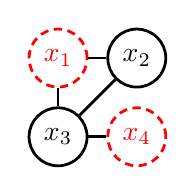
\begin{tikzpicture}[line width=1pt,node distance=14mm ,main/.style = {draw, circle},scale=1] 
   \node[main,color=red,densely dashed] at (0,1) (x1) {\texttt{$x_1$}};
   \node[main,color=black] at (1,1) (x2) {\texttt{$x_2$}};
       \node[main,color=black] at (0,0) (x3) {\texttt{$x_3$}};
       \node[main,color=red,densely dashed] at (1,0) (x4) {\texttt{$x_4$}};
      \draw (x1) -- (x2);
       \draw (x1) -- (x3);
      \draw (x2) -- (x3);
      \draw (x3) -- (x4);
   \end{tikzpicture}
       };
   
   \node[scale=.8] at (7,5.5){$\textup{PerfMatch}[b,\{x_1,x_2\}]$};
       \node[main] at (7,4) (9) {
   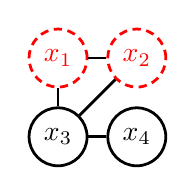
\begin{tikzpicture}[line width=1pt,node distance=14mm ,main/.style = {draw, circle},scale=1] 
   \node[main,color=red,densely dashed] at (0,1) (x1) {\texttt{$x_1$}};
   \node[main,color=red,densely dashed] at (1,1) (x2) {\texttt{$x_2$}};
       \node[main,color=black] at (0,0) (x3) {\texttt{$x_3$}};
       \node[main,color=black] at (1,0) (x4) {\texttt{$x_4$}};
      \draw (x1) -- (x2);
       \draw (x1) -- (x3);
      \draw (x2) -- (x3);
      \draw (x3) -- (x4);
   \end{tikzpicture}
       };
       
    \node[scale=.8] at (0,1.5){$\textup{PerfMatch}[c,\{x_2,x_3,x_4\}]$};
       \node[main] at (0,0) (8) {
   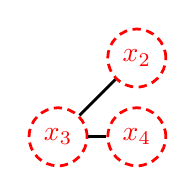
\begin{tikzpicture}[line width=1pt,node distance=14mm ,main/.style = {draw, circle},scale=1] 
   \node[main,color=red,densely dashed] at (1,1) (x2) {\texttt{$x_2$}};
       \node[main,color=red,densely dashed] at (0,0) (x3) {\texttt{$x_3$}};
       \node[main,color=red,densely dashed] at (1,0) (x4) {\texttt{$x_4$}};
      \draw (x2) -- (x3);
      \draw (x3) -- (x4);
   \end{tikzpicture}
   };
   
    \node[scale=.8] at (3.5,1.5){$\textup{PerfMatch}[c,\{x_4\}]$};
   \node[main] at (3.5,0) (8) {
   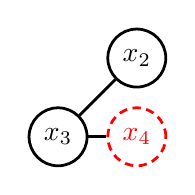
\begin{tikzpicture}[line width=1pt,node distance=14mm ,main/.style = {draw, circle},scale=1] 
   \node[main,color=black] at (1,1) (x2) {\texttt{$x_2$}};
       \node[main,color=black] at (0,0) (x3) {\texttt{$x_3$}};
       \node[main,color=red,densely dashed] at (1,0) (x4) {\texttt{$x_4$}};
      \draw (x2) -- (x3);
      \draw (x3) -- (x4);
   \end{tikzpicture}
   };
   
    \node[scale=.8] at (7,1.5){$\textup{PerfMatch}[c,\{x_2\}]$};
   \node[main] at (7,0) (8) {
   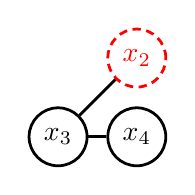
\begin{tikzpicture}[line width=1pt,node distance=14mm ,main/.style = {draw, circle},scale=1] 
   \node[main,color=red,densely dashed] at (1,1) (x2) {\texttt{$x_2$}};
       \node[main,color=black] at (0,0) (x3) {\texttt{$x_3$}};
       \node[main,color=black] at (1,0) (x4) {\texttt{$x_4$}};
      \draw (x2) -- (x3);
      \draw (x3) -- (x4);
   \end{tikzpicture}
   };
   
   
   
       \draw [->](0,2) -- (0,2.5);
       \draw [->](3.5,2) -- (3.5,2.5);
       \draw [->](7,2) -- (7,2.5);
   
   
    \node[scale=.8] at (10.5,5.5){$\textup{PerfMatch}[b,\{x_3,x_4\}]$};
       \node[main] at (10.5,4) (9) {
   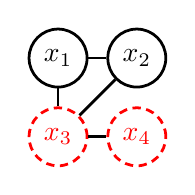
\begin{tikzpicture}[line width=1pt,node distance=14mm ,main/.style = {draw, circle},scale=1] 
   \node[main,color=black] at (0,1) (x1) {\texttt{$x_1$}};
   \node[main,color=black] at (1,1) (x2) {\texttt{$x_2$}};
       \node[main,color=red,densely dashed] at (0,0) (x3) {\texttt{$x_3$}};
       \node[main,color=red,densely dashed] at (1,0) (x4) {\texttt{$x_4$}};
      \draw (x1) -- (x2);
       \draw (x1) -- (x3);
      \draw (x2) -- (x3);
      \draw (x3) -- (x4);
   \end{tikzpicture}
       };
   
       \draw [->](10.5,1) -- (10.5,2.5);
       \node[scale=3] at (10.5,0){$\varnothing$};
       %\node[text width=6cm] at (2,-2){$\DP[i,c]$};
       %\node[text width=6cm] at (5.5,-2){$\DP[i,c+\{x_4\to \texttt{gray/dotted}]$};
      
   \end{tikzpicture}
   }}
\end{figure}

\begin{figure}[H]
	\floatbox[{\capbeside\thisfloatsetup{capbesideposition={right,top},capbesidewidth=5cm}}]{figure}[\FBwidth]
	{\caption{Computing values in forget nodes. Bag $b$ forgets node $x_1$ and has child $c$. Notice that nodes $x_2$ and $x_3$ have been matched with some element not in $X_b$. Since we consider a perfect matching, $x_1$ must have been matched before being forgotten. We thus consider the cases where $x_1$ was already matched in $c$, where $x_1$ matched with $x_2$ and where $x_1$ matched with $x_3$.
		}\label{fig:forget_node}}
	{\resizebox{0.58\textwidth}{!}{% !TEX root = ../main.tex
\begin{tikzpicture}[line width=1pt,node distance=14mm ,main/.style = {draw, rectangle},scale=1] 

    \node[scale=.8] at (3,6){$\textup{PerfMatch}[b,\{x_4\}]$};
       
       \node[main] at (3,4.5) (9) {
   \begin{tikzpicture}[line width=1pt,node distance=14mm ,main/.style = {draw, circle},scale=1] 
   \node[main,color=black] at (1,1) (x2) {\texttt{$x_2$}};
       \node[main,color=black] at (0,0) (x3) {\texttt{$x_3$}};
       \node[main,fill=red!40!white,densely dashed] at (1,0) (x4) {\texttt{$x_4$}};
      \draw (x2) -- (x3);
      \draw (x3) -- (x4);
   \end{tikzpicture}
       };
       
    \node[scale=.8] at (-1,1.5){$\textup{PerfMatch}[c,\{x_4\}]$};
       \node[main] at (-1,0) (8) {
   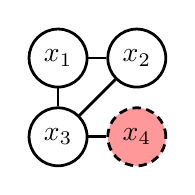
\begin{tikzpicture}[line width=1pt,node distance=14mm ,main/.style = {draw, circle},scale=1] 
   \node[main,color=black] at (0,1) (x1) {\texttt{$x_1$}};
   \node[main,color=black] at (1,1) (x2) {\texttt{$x_2$}};
       \node[main,color=black] at (0,0) (x3) {\texttt{$x_3$}};
       \node[main,fill=red!40!white,densely dashed] at (1,0) (x4) {\texttt{$x_4$}};
      \draw (x1) -- (x2);
       \draw (x1) -- (x3);
      \draw (x2) -- (x3);
      \draw (x3) -- (x4);
   \end{tikzpicture}
   };
   
    \node[scale=.8] at (3,1.5){$\textup{PerfMatch}[c,\{x_4\}\cup \{x_1,x_2\}]$};
   \node[main] at (3,0) (8) {
   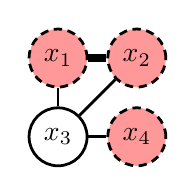
\begin{tikzpicture}[line width=1pt,node distance=14mm ,main/.style = {draw, circle},scale=1] 
   \node[main,fill=red!40!white,densely dashed] at (0,1) (x1) {\texttt{$x_1$}};
   \node[main,fill=red!40!white,densely dashed] at (1,1) (x2) {\texttt{$x_2$}};
       \node[main,color=black] at (0,0) (x3) {\texttt{$x_3$}};
       \node[main,fill=red!40!white,densely dashed] at (1,0) (x4) {\texttt{$x_4$}};
      \draw [line width = 3pt, color=black]  (x1) -- (x2);
       \draw (x1) -- (x3);
      \draw (x2) -- (x3);
      \draw (x3) -- (x4);
   \end{tikzpicture}
   };
   
    \node[scale=.8] at (7,1.5){$\textup{PerfMatch}[c,\{x_4\}\cup \{x_1,x_3\}]$};
   \node[main] at (7,0) (8) {
   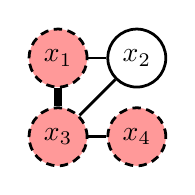
\begin{tikzpicture}[line width=1pt,node distance=14mm ,main/.style = {draw, circle},scale=1] 
   \node[main,fill=red!40!white,densely dashed] at (0,1) (x1) {\texttt{$x_1$}};
   \node[main,color=black] at (1,1) (x2) {\texttt{$x_2$}};
       \node[main,fill=red!40!white,densely dashed] at (0,0) (x3) {\texttt{$x_3$}};
       \node[main,fill=red!40!white,densely dashed] at (1,0) (x4) {\texttt{$x_4$}};
      \draw (x1) -- (x2);
       \draw [line width = 3pt, color=black] (x1) -- (x3);
      \draw (x2) -- (x3);
      \draw (x3) -- (x4);
   \end{tikzpicture}
   };
   
       \draw [decorate,decoration={brace,amplitude=10}] (0,2.5) -- (6,2.5) node [black,midway,xshift=-0.6cm] {};
   
       %\node[text width=6cm] at (2,-2){$\DP[i,c]$};
       %\node[text width=6cm] at (5.5,-2){$\DP[i,c+\{x_4\to \texttt{gray/dotted}]$};
      
   \end{tikzpicture}
   }}
\end{figure}

\begin{figure}[H]
	\floatbox[{\capbeside\thisfloatsetup{capbesideposition={right,top},capbesidewidth=5cm}}]{figure}[\FBwidth]
	{\caption{Computing the values at join nodes. Bag $b$ has children $c_1$ and $c_2$. Nodes $x_3$ and $x_4$ have been matched with elements not in $b$, but these elements could have been in the subtree of $c_1$ or the subtree of $c_2$. We thus iterate over all possible ways to distribute these matched nodes between $c_1$ and $c_2$. For each of these ways, we multiply the number of respectful matchings in $c_1$ and $c_2$, then, finally, we add these results together to find the answer for $b$.
		}\label{fig:join_node}}
	{\resizebox{0.6\textwidth}{!}{% !TEX root = ../main.tex
\begin{tikzpicture}[line width=1pt,node distance=14mm ,main/.style = {draw, rectangle},scale=1] 

    \node[scale=.8] at (-4,1){$\textup{PerfMatch}[b,\{x_1,x_4\}]$};
       \node[main] at (-4,-0.5) (9) {
   \begin{tikzpicture}[line width=1pt,node distance=14mm ,main/.style = {draw, circle},scale=1] 
   \node[main,fill=red!40!white,densely dashed] at (0,1) (x1) {\texttt{$x_1$}};
   \node[main,color=black] at (1,1) (x2) {\texttt{$x_2$}};
       \node[main,color=black] at (0,0) (x3) {\texttt{$x_3$}};
       \node[main,fill=red!40!white,densely dashed] at (1,0) (x4) {\texttt{$x_4$}};
      \draw  (x1) -- (x2);
       \draw (x1) -- (x3);
      \draw (x2) -- (x3);
      \draw (x3) -- (x4);
   \end{tikzpicture}
       };
       
    \node[scale=.8] at (0,5.5){$\textup{PerfMatch}[c_1,\{x_1,x_4\}\cup \{x_2,x_3\}]$};
       \node[main] at (0,4) (8) {
   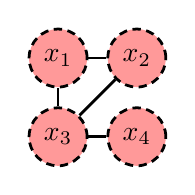
\begin{tikzpicture}[line width=1pt,node distance=14mm ,main/.style = {draw, circle},scale=1] 
   \node[main,fill=red!40!white,densely dashed] at (0,1) (x1) {\texttt{$x_1$}};
   \node[main,fill=red!40!white,densely dashed] at (1,1) (x2) {\texttt{$x_2$}};
       \node[main,fill=red!40!white,densely dashed] at (0,0) (x3) {\texttt{$x_3$}};
       \node[main,fill=red!40!white,densely dashed] at (1,0) (x4) {\texttt{$x_4$}};
      \draw (x1) -- (x2);
       \draw (x1) -- (x3);
      \draw (x2) -- (x3);
      \draw (x3) -- (x4);
   \end{tikzpicture}
   };
   
    \node[scale=3] at (2,4){$\cdot$};
   
    \node[scale=.8] at (4,5.5){$\textup{PerfMatch}[c_2,\{x_1,x_4\}\cup \{\}]$};
   \node[main] at (4,4) (8) {
   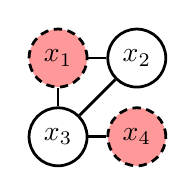
\begin{tikzpicture}[line width=1pt,node distance=14mm ,main/.style = {draw, circle},scale=1] 
   \node[main,fill=red!40!white,densely dashed] at (0,1) (x1) {\texttt{$x_1$}};
   \node[main,color=black] at (1,1) (x2) {\texttt{$x_2$}};
       \node[main,color=black] at (0,0) (x3) {\texttt{$x_3$}};
       \node[main,fill=red!40!white,densely dashed] at (1,0) (x4) {\texttt{$x_4$}};
      \draw (x1) -- (x2);
       \draw (x1) -- (x3);
      \draw (x2) -- (x3);
      \draw (x3) -- (x4);
   \end{tikzpicture}
   };
   
    \node[scale=.8] at (0,2.5){$\textup{PerfMatch}[c_1,\{x_1,x_4\}\cup \{x_3\}]$};
   \node[main] at (0,1) (8) {
   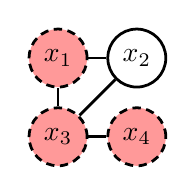
\begin{tikzpicture}[line width=1pt,node distance=14mm ,main/.style = {draw, circle},scale=1] 
   \node[main,fill=red!40!white,densely dashed] at (0,1) (x1) {\texttt{$x_1$}};
   \node[main,color=black] at (1,1) (x2) {\texttt{$x_2$}};
       \node[main,fill=red!40!white,densely dashed] at (0,0) (x3) {\texttt{$x_3$}};
       \node[main,fill=red!40!white,densely dashed] at (1,0) (x4) {\texttt{$x_4$}};
      \draw (x1) -- (x2);
       \draw (x1) -- (x3);
      \draw (x2) -- (x3);
      \draw (x3) -- (x4);
   \end{tikzpicture}
   };
   
    \node[scale=3] at (2,1){$\cdot$};
   
    \node[scale=.8] at (4,2.5){$\textup{PerfMatch}[c_2,\{x_1,x_4\}\cup \{x_2\}]$};
   \node[main] at (4,1) (8) {
   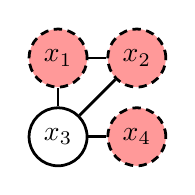
\begin{tikzpicture}[line width=1pt,node distance=14mm ,main/.style = {draw, circle},scale=1] 
   \node[main,fill=red!40!white,densely dashed] at (0,1) (x1) {\texttt{$x_1$}};
   \node[main,fill=red!40!white,densely dashed] at (1,1) (x2) {\texttt{$x_2$}};
       \node[main,color=black] at (0,0) (x3) {\texttt{$x_3$}};
       \node[main,fill=red!40!white,densely dashed] at (1,0) (x4) {\texttt{$x_4$}};
      \draw (x1) -- (x2);
       \draw (x1) -- (x3);
      \draw (x2) -- (x3);
      \draw (x3) -- (x4);
   \end{tikzpicture}
   };
   
    \node[scale=.8] at (0,-0.5){$\textup{PerfMatch}[c_1,\{x_1,x_4\}\cup \{x_2\}]$};
   \node[main] at (0,-2) (8) {
   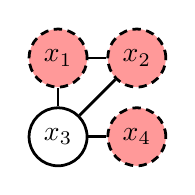
\begin{tikzpicture}[line width=1pt,node distance=14mm ,main/.style = {draw, circle},scale=1] 
   \node[main,fill=red!40!white,densely dashed] at (0,1) (x1) {\texttt{$x_1$}};
   \node[main,fill=red!40!white,densely dashed] at (1,1) (x2) {\texttt{$x_2$}};
       \node[main,color=black] at (0,0) (x3) {\texttt{$x_3$}};
       \node[main,fill=red!40!white,densely dashed] at (1,0) (x4) {\texttt{$x_4$}};
      \draw (x1) -- (x2);
       \draw (x1) -- (x3);
      \draw (x2) -- (x3);
      \draw (x3) -- (x4);
   \end{tikzpicture}
   };
   
    \node[scale=3] at (2,-2){$\cdot$};
   
    \node[scale=.8] at (4,-0.5){$\textup{PerfMatch}[c_2,\{x_1,x_4\}\cup \{x_3\}]$};
   \node[main] at (4,-2) (8) {
   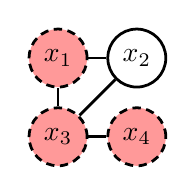
\begin{tikzpicture}[line width=1pt,node distance=14mm ,main/.style = {draw, circle},scale=1] 
   \node[main,fill=red!40!white,densely dashed] at (0,1) (x1) {\texttt{$x_1$}};
   \node[main,color=black] at (1,1) (x2) {\texttt{$x_2$}};
       \node[main,fill=red!40!white,densely dashed] at (0,0) (x3) {\texttt{$x_3$}};
       \node[main,fill=red!40!white,densely dashed] at (1,0) (x4) {\texttt{$x_4$}};
      \draw (x1) -- (x2);
       \draw (x1) -- (x3);
      \draw (x2) -- (x3);
      \draw (x3) -- (x4);
   \end{tikzpicture}
   };
   
    \node[scale=.8] at (0,-3.5){$\textup{PerfMatch}[c_1,\{x_1,x_4\}\cup \{\}]$};
   \node[main] at (0,-5) (8) {
   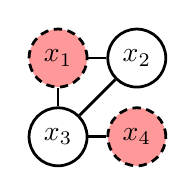
\begin{tikzpicture}[line width=1pt,node distance=14mm ,main/.style = {draw, circle},scale=1] 
   \node[main,fill=red!40!white,densely dashed] at (0,1) (x1) {\texttt{$x_1$}};
   \node[main,color=black] at (1,1) (x2) {\texttt{$x_2$}};
       \node[main,color=black] at (0,0) (x3) {\texttt{$x_3$}};
       \node[main,fill=red!40!white,densely dashed] at (1,0) (x4) {\texttt{$x_4$}};
      \draw (x1) -- (x2);
       \draw (x1) -- (x3);
      \draw (x2) -- (x3);
      \draw (x3) -- (x4);
   \end{tikzpicture}
   };
   
    \node[scale=3] at (2,-5){$\cdot$};
   
     \node[scale=.8] at (4,-3.5){$\textup{PerfMatch}[c_2,\{x_1,x_4\}\cup \{x_2,x_3\}]$};
   \node[main] at (4,-5) (8) {
   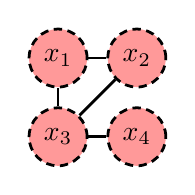
\begin{tikzpicture}[line width=1pt,node distance=14mm ,main/.style = {draw, circle},scale=1] 
   \node[main,fill=red!40!white,densely dashed] at (0,1) (x1) {\texttt{$x_1$}};
   \node[main,fill=red!40!white,densely dashed] at (1,1) (x2) {\texttt{$x_2$}};
       \node[main,fill=red!40!white,densely dashed] at (0,0) (x3) {\texttt{$x_3$}};
       \node[main,fill=red!40!white,densely dashed] at (1,0) (x4) {\texttt{$x_4$}};
      \draw (x1) -- (x2);
       \draw (x1) -- (x3);
      \draw (x2) -- (x3);
      \draw (x3) -- (x4);
   \end{tikzpicture}
   };
   
       \draw [decorate,decoration={brace,amplitude=10}] (-2,-5) -- (-2,4) node [black,midway,xshift=-0.6cm] {};
   
       %\draw [->](-2,3.5) -- (-3,2.5);
       %\draw [->](-2,1) -- (-3,0.5);
       %\draw [->](-2,-2) -- (-3,-1.5);
       %\draw [->](-2,-4.5) -- (-3,-3.5);
       %\draw [->](3.5,-2.5) -- (5,-3);
       %\draw [->](3.5,-5) -- (5,-4.5);
       %\draw [->](3.5,-7.5) -- (5,-6);
       %\node[text width=6cm] at (2,-2){$\DP[i,c]$};
       %\node[text width=6cm] at (5.5,-2){$\DP[i,c+\{x_4\to \texttt{gray/dotted}]$};
      
   \end{tikzpicture}}}
\end{figure}

\subsection{Illustrative Figures for Dynamic Programming in Matching Computation (Hosoya Index)}
\label{appendix:figure_matching}
\begin{figure}[H]
	\caption{Computing values in forget nodes. Cases for introduce and merge nodes are the same as to \ref{subsec:perfect_pathwidth}, represented in \ref{fig:introduce_node} and \ref{fig:join_node}, respectively. Forget nodes need to consider one more case when compared to \ref{fig:forget_node}, represented by the second case below bag $b$. This is when $x_1$ remains unmatched, since we do not need to generate a perfect matching.
	}\label{fig:forget_node_matching}
	{\resizebox{0.63\textwidth}{!}{% !TEX root = ../main.tex
\begin{tikzpicture}[line width=1pt,node distance=14mm ,main/.style = {draw, rectangle},scale=1] 

    \node[scale=.8] at (3.15,6){$\textup{Match}[b,\{x_4\}]$};
       
       \node[main] at (3.15,4.5) (9) {
   \begin{tikzpicture}[line width=1pt,node distance=14mm ,main/.style = {draw, circle},scale=1] 
   \node[main,color=black] at (1,1) (x2) {\texttt{$x_2$}};
       \node[main,color=black] at (0,0) (x3) {\texttt{$x_3$}};
       \node[main,fill=blue!40!white,densely dashed] at (1,0) (x4) {\texttt{$x_4$}};
      \draw (x2) -- (x3);
      \draw (x3) -- (x4);
   \end{tikzpicture}
       };
       
    \node[scale=.8] at (-1.5,1.5){$\textup{Match}[c,\{x_4\}]$};
       \node[main] at (-1.5,0) (8) {
   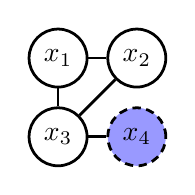
\begin{tikzpicture}[line width=1pt,node distance=14mm ,main/.style = {draw, circle},scale=1] 
   \node[main,color=black] at (0,1) (x1) {\texttt{$x_1$}};
   \node[main,color=black] at (1,1) (x2) {\texttt{$x_2$}};
       \node[main,color=black] at (0,0) (x3) {\texttt{$x_3$}};
       \node[main,fill=blue!40!white,densely dashed] at (1,0) (x4) {\texttt{$x_4$}};
      \draw (x1) -- (x2);
       \draw (x1) -- (x3);
      \draw (x2) -- (x3);
      \draw (x3) -- (x4);
   \end{tikzpicture}
   };
   
    \node[scale=.8] at (1.3,1.5){$\textup{Match}[c,\{x_4\}\cup \{x_1\}]$};
   \node[main] at (1.3,0) (8) {
   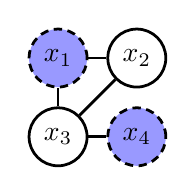
\begin{tikzpicture}[line width=1pt,node distance=14mm ,main/.style = {draw, circle},scale=1] 
   \node[main,fill=blue!40!white,densely dashed] at (0,1) (x1) {\texttt{$x_1$}};
   \node[main,color=black] at (1,1) (x2) {\texttt{$x_2$}};
       \node[main] at (0,0) (x3) {\texttt{$x_3$}};
       \node[main,fill=blue!40!white,densely dashed] at (1,0) (x4) {\texttt{$x_4$}};
      \draw (x1) -- (x2);
       \draw (x1) -- (x3);
      \draw (x2) -- (x3);
      \draw (x3) -- (x4);
   \end{tikzpicture}
   };
   
    \node[scale=.8] at (4.5,1.5){$\textup{Match}[c,\{x_4\}\cup \{x_1,x_2\}]$};
   \node[main] at (4.5 ,0) (8) {
   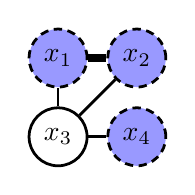
\begin{tikzpicture}[line width=1pt,node distance=14mm ,main/.style = {draw, circle},scale=1] 
   \node[main,fill=blue!40!white,densely dashed] at (0,1) (x1) {\texttt{$x_1$}};
   \node[main,fill=blue!40!white,densely dashed] at (1,1) (x2) {\texttt{$x_2$}};
       \node[main,color=black] at (0,0) (x3) {\texttt{$x_3$}};
       \node[main,fill=blue!40!white,densely dashed] at (1,0) (x4) {\texttt{$x_4$}};
      \draw [line width = 3pt, color=black]  (x1) -- (x2);
       \draw (x1) -- (x3);
      \draw (x2) -- (x3);
      \draw (x3) -- (x4);
   \end{tikzpicture}
   };

   \node[scale=.8] at (7.8,1.5){$\textup{Match}[c,\{x_4\}\cup \{x_1,x_3\}]$};
   \node[main] at (7.8,0) (8) {
   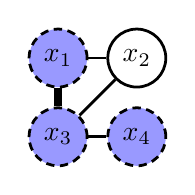
\begin{tikzpicture}[line width=1pt,node distance=14mm ,main/.style = {draw, circle},scale=1] 
   \node[main,fill=blue!40!white,densely dashed] at (0,1) (x1) {\texttt{$x_1$}};
   \node[main,color=black] at (1,1) (x2) {\texttt{$x_2$}};
       \node[main,fill=blue!40!white,densely dashed] at (0,0) (x3) {\texttt{$x_3$}};
       \node[main,fill=blue!40!white,densely dashed] at (1,0) (x4) {\texttt{$x_4$}};
      \draw (x1) -- (x2);
       \draw [line width = 3pt, color=black] (x1) -- (x3);
      \draw (x2) -- (x3);
      \draw (x3) -- (x4);
   \end{tikzpicture}
   };
   
       \draw [decorate,decoration={brace,amplitude=10}] (-1.5,2.5) -- (7.8,2.5) node [black,midway,xshift=-0.6cm] {};
   
       %\node[text width=6cm] at (2,-2){$\DP[i,c]$};
       %\node[text width=6cm] at (5.5,-2){$\DP[i,c+\{x_4\to \texttt{gray/dotted}]$};
      
   \end{tikzpicture}
   }}
\end{figure}


\subsection{Figure Illustrating Proposition \ref{prop:comp_tw_matchings_size_k}}
\begin{figure}[H]
	\resizebox{0.32\textwidth}{!}{% !TEX root = ../main.tex
% \begin{center}
\begin{tikzpicture}[node distance={17mm}, thick, main/.style = {draw, rectangle split,rectangle split parts=2}] 
\node[main] (0) []{ $n_b = 72$ \nodepart{two}$x_1,x_2,x_3$}; 
\node[main] (00) [below left of =0]{ $n_b = 40$ \nodepart{two}$x_1,x_2,x_3$};
\node[] (000) [below of =00,node distance={8mm}]{...};

\node[main,fill=cyan!20, dashed] (01) [below right of =0]{$n_b = 35$ \nodepart{two}$x_1,x_2,x_3$};
\node[] (010) [below of =01,node distance={8mm}]{...};
\node[main] (011) [below of =010,node distance={8mm}]{$n_b = 29$ \nodepart{two}$x_1,x_{10},x_{11}$};
\node[main] (0110) [below left of =011]{$n_b = 20$ \nodepart{two}$x_1,x_{10},x_{11}$};
\node[] (0110p) [below of =0110,node distance={8mm}]{...};
\node[main,fill=cyan!20, dashed] (0111) [below right of =011]{$n_b = 12$ \nodepart{two}$x_1,x_{10},x_{11}$};
\node[] (0111p) [below of =0111,node distance={8mm}]{...};
\node[main] (01110) [below of =0111p,,node distance={8mm}]{$n_b = 6$ \nodepart{two}$x_{10},\textcolor{red}{x_{15}}$};
\node[] (01110p) [below of =01110,node distance={8mm}]{...};

\draw [] (0) -- (00); 
\draw [] (00) -- (000); 

\draw [line width=3pt] (0) -- (01); 
\draw [] (01) -- (010); 
\draw [] (010) -- (011); 

\draw [line width=3pt] (011) -- (0111); 
\draw [] (011) -- (0110); 
\draw [] (0110) -- (0110p); 

\draw [] (0111) -- (0111p); 
\draw [] (0111p) -- (01110); 

\draw [] (01110) -- (01110p); 


\end{tikzpicture}
% \end{center}}
	\caption{This figure illustrates Proposition \ref{prop:comp_tw_matchings_size_k}. The tree shown represents a nice tree decomposition. Sequences of forget and introduce nodes have been omitted by ``...''. Bags in $L$, or bags that are the light child of some join bag, have been highlighted in blue (dashed). Notice that each of these bags has a parent $b$ with weight $n_b$ at least $1.5$ times the weight of its lightest child. Thus, a node, such as $x_{15}$, highlighted in red, can have at most $\log n$ light ancestors.
	}
	\label{fig:log_tree}
	
\end{figure}

\paragraph{Implementation}
We implemented our algorithms, as well as those of~\cite{wan2018computing} and the naive brute-force approaches (See \ref{app:brute}), in \texttt{C++}. We used FlowCutter~\cite{strasser2017computing} to obtain the tree decompositions. The implementation will be published as free and open-source software in the public domain and with no copyright.

\paragraph{Machine}
All experimental results were obtained on an Intel Xeon Gold 5115 Machine (2.40GHz, 16 cores) with 64 GB of RAM, running Ubuntu 22.04. The computations took approximately three days to complete. 



%\section{Naive Baseline Algorithms} 
%We now provide a brief treatment for naive baseline algorithms for computing total number of perfect matchings, matchings and independent set. We also provide complextiy analysis for them. We used these baseline algorithms as one of the benchmarks for our experiments and give a detailed comparision with our algorithms in Section \ref{sec:Experiments}.



\paragraph{Naive Baseline Algorithms} We also provide naive non-parameterized algorithms for the problems considered in this work. These are the non-parameterized algorithms used in our experimental results. The parameterized baselines were taken from~\cite{wan2018computing}. We denote the numbers of perfect matchings, matchings and indpendent sets of $G$ by $\pma(G), \ma(G)$ and $\ind(G)$ respectively. We obtain all of these values by dynamic programming using the following recurrences.

% \begin{notation}
	% Let $W$ be a set of vertices $G$, by $G \setminus W$ we denote a graph $G \setminus W = G[V(G) \setminus W]$. If $e \in E(G)$ by
	% 	$G - e$ we demote a new graph $G - e := (V(G), E(G)\setminus e)$. By $N[v]$ we denote closed neighbourhood of a vertex $v$.
	% \end{notation}

% Naive algorithms are based on recursive formulas for the corresponding graph structures. 
% For a graph $G$, denote by $\pma(G)$, $\ma(G)$, $\ind(G)$ the number of perfect matchings, the number of matchings, and the number of independent subsets, 
% respectively.
% We will now present the baseline algorithms for computing perfect matchings, matchings and independent sets:


	\[
	\pma(G) =
	\begin{cases}
		\pma(G - \{u, v\}) + 
		\pma(G - uv) & uv \in E(G)  \\
		1 & E(G) = V(G) = \emptyset \\
		0 & E(G) = \emptyset, V(G) \neq \emptyset
	\end{cases}
	\]
	

	\[
	\ma(G) =
	\begin{cases}
			\ma(G - \{u, v\}) + \ma(G - uv) & uv \in E(G) \\
		1 & E(G) = \emptyset\\
	\end{cases}
	\]
	

	\[
	\ind(G) =
	\begin{cases}
		\ind(G - N[v]) + \ind(G - v) & E(G) \neq \emptyset \\
		2^{\abs{V(G)}} & E(G) = \emptyset
	\end{cases}
	\]


%\begin{theorem}\label{thm:naive_baseline}
%	% Let $E(G) \neq \varnothing$, then $(u, v) \in E(G)$.
%	Let $G$ be the graph with $\abs{E(G)} = m$ and $\abs{V(G)} = n$, then the time complexity for computing all the above recurrence relations is $\bigO(2^{m} \cdot \textup{poly}(n))$.
%\end{theorem}
%% \begin{proof}
%	% 	The above mentioned baseline algorithms implement the following branching strategy: Consider an arbitrary edge or vertex of the graph $G$. Now we get a choice for it i.e., whether it belongs to the structure we are counting or not. This implies that branching for the above mentioned recurrence formulas have degree at most two. Also, observe that after execution of each branch the number of edges of graph decrease by at least one. Therefore, the depth of the recursion trees is at most $m$, and the number of leaves of the recursion trees are at most $2 ^ {m}$. Hence, completing the proof that the time complexity for all the above mentioned baseline algorithms is $\bigO(2^{m} \cdot \textup{poly}(n))$.
%	% \end{proof}
%
%\begin{proof}
%	The above mentioned baseline algorithms implement the following branching strategy: Consider an arbitrary edge or vertex of the graph $G$. Now we get a choice for it i.e., whether it belongs to the structure we are counting or not. This implies that branching for the above mentioned recurrence formulas have degree at most two. Also, observe that after execution of each branch the number of edges of graph decrease by at least one. Therefore, the depth of the recursion trees is at most $m$, and the number of leaves of the recursion trees are at most $2 ^ {m}$. Hence, completing the proof that the time complexity for all the above mentioned baseline algorithms is $\bigO(2^{m} \cdot \textup{poly}(n))$.
%\end{proof}

\newpage